\documentclass{book}
\usepackage{amsmath}
\usepackage{bm}
\usepackage{colortbl}
\usepackage{graphicx}
\usepackage{caption}
\usepackage{fullpage}
\usepackage{afterpage}
\usepackage{multirow}
\usepackage[nodisplayskipstretch]{setspace}
\usepackage{booktabs}
\usepackage{gensymb}
\usepackage{parskip}
\usepackage{xr}
\usepackage{pdflscape}
\usepackage[labelfont=bf,tableposition=top]{caption}
\usepackage[inline]{enumitem}
\usepackage{wrapfig}
\usepackage{longtable}
\usepackage{subfig}
\usepackage[natbib=true,subentry,backend=biber,sorting=none,citestyle=authoryear-comp]{biblatex}
\addbibresource{citation/Thesis.bib}
\usepackage[hidelinks]{hyperref}
\usepackage{geometry}
\geometry{
	top=1in,            % <-- you want to adjust this
	inner=1in,
	outer=1in,
	bottom=1in,
	headheight=3ex,       % <-- and this
	headsep=2ex,          % <-- and this
}
\usepackage{fancyhdr}
\usepackage{fixltx2e}
\usepackage[acronym,nomain,toc,makeindex ]{glossaries}
\usepackage{cleveref} %This need to be the last package for it to work properly 
\newcommand{\beginsupplement}{%
	\setcounter{table}{0}
	\renewcommand{\thetable}{S\arabic{table}}%
	\setcounter{figure}{0}
	\renewcommand{\thefigure}{S\arabic{figure}}%
}

\pagestyle{fancy}
\fancyhf{}
\fancyfoot[LE,RO]{\thepage}
\renewcommand{\footrulewidth}{1pt}
\fancyhead[L]{\leftmark}
\fancyhead[R]{\rightmark}
\title{Genetic and Environmental risk factors of Schizophrenia and Autism}
\date{\today}
\author{\href{mailto:choishingwan@gmail.com}{Choi Shing Wan}\\
	
\includegraphics[width=0.5\textwidth]{hkuLogo.jpg}}
\singlespacing
\renewcommand*\contentsname{Contents}
\onehalfspacing
%\doublespacing

%\includeonly{environmental_risk/er_chapter,supplementary_materials}

\makeglossary
\newacronym{SCZ}{SCZ}{Schizophrenia}
\newacronym{ASD}{ASD}{Autism Spectrum Disorder}
\newacronym[longplural={Genome Wide Association Studies}]{GWAS}{GWAS}{Genome Wide Association Study}
\newacronym{wgs}{WGS}{Whole Genome Sequencing}
\newacronym{SNP}{SNP}{Single Nucleotide Polymorphism}
\newacronym{LD}{LD}{Linkage Disequilibrium}
\newacronym{PGS}{PGS}{Polygenic Risk Score}
\newacronym{tSVD}{tSVD}{Truncated Singular Value Decomposition}
\newacronym{SVD}{SVD}{Singular Value Decomposition}
\newacronym{shrek}{SHREK}{SNP Heritability and Risk Estimation Kit}
\newacronym{gcta}{GCTA}{Genome-wide Complex Trait Analysis}
\newacronym{ldsc}{LDSC}{LD SCore}
\newacronym{CEU}{CEU}{Northern Europeans from Utah}
\newacronym{se}{SE}{Standard Error}
\newacronym{maf}{maf}{Minor Allele Frequency}
\newacronym{pgc}{PGC}{Psychiatric Genomics Consortium}
\newacronym{rin}{RIN}{RNA integrity number}
\newacronym{gd}{GD}{Gestation Day}
\newacronym{rpkm}{RPKM}{Reads Per Kilobase per Million mapped reads}
\newacronym{wgcna}{WGCNA}{Weighted Gene Co-expression Network Analysis}
\newacronym{pc}{PC}{Principle Component}
\newacronym{GO}{GO}{Gene Ontology}
\newacronym{MAGMA}{MAGMA}{Multi-marker Analysis of GenoMic Annotation}
\newacronym{ngs}{NGS}{Next Generation Sequencing}
%\raggedbottom %Remove it before printing as this is something to do with global settings. Can make each page look uneven but more dense. 
\makeindex
\begin{document}\thispagestyle{empty}
\pagestyle{empty}

%\maketitle
\begin{titlepage}
	\begin{center}
		\vspace*{1cm}
		
		\Huge
		\textbf{Heritability Estimation and Risk Prediction in Schizophrenia}
		
		\vspace{0.5cm}
		\LARGE
		
		\vspace{1.5cm}
		
		\textbf{\href{mailto:choishingwan@gmail.com}{Choi Shing Wan}}
		
		\vfill
		
		A thesis submitted in partial fulfillment of the requirements for \\
		the Degree of Doctor of Philosophy
		
		\vspace{0.8cm}
		
		
\includegraphics[width=0.4\textwidth]{figure/hkuLogo.jpg}
		
		\Large
		Department of Psychiatry\\
		University of Hong Kong\\
		Hong Kong\\
		\today
		
	\end{center}
\end{titlepage}


\frontmatter 

	\cleardoublepage
	\phantomsection
	\addcontentsline{toc}{chapter}{Declaration}
	\newgeometry{inner=2in, outer=2in}
	\chapter*{\centerline{Declaration}}
	\vspace{1cm}
	I declare that this thesis represents my own work, except where due acknowledgments	is made, and that it has not been previously included in a thesis, dissertation or report submitted to this University or to any other institution for a degree,	diploma or other qualification.
	\vspace{1.5cm}
	
	\centerline{Signed....................................................................}
	\restoregeometry
	\cleardoublepage
	\phantomsection
	\addcontentsline{toc}{chapter}{Acknowledgments}
	\chapter*{\centerline{Acknowledgements}}
	\cleardoublepage
	\phantomsection
	\begin{singlespace}
	\printglossary[title=Abbreviations,toctitle=Abbreviations]
	\cleardoublepage
	\phantomsection
	%To generate the correct abbreviations, use alt+shift+F1 twice before using F1
	
	\cleardoublepage
	\phantomsection
	\addcontentsline{toc}{chapter}{Contents}
		\tableofcontents
		\listoffigures
		\listoftables
	\end{singlespace}
\mainmatter
\pagestyle{fancy}
	\chapter{Introduction}
		%\addcontentsline{toc}{chapter}{Introduction}
	\chapter*{Some considerations}
	\begin{enumerate}
		\item PRSice requires the phenotype to aid its selection (More information= stronger)
		\item It seems like LDSC doesn't necessary perform badly in oligogenic situation.
		Rather, it is that when the trait is oligogenic, it is more likely for LDSC to behaviour in a strange way.
		\item For each condition: extreme phenotype, quantitative trait, case control, we can have a separated review. 
		Discuss on the benefits and challenges of each condition and the method we deal with them.
		So we can have two chapters (case control, quantitative trait) where extreme phenotype can be a big subsection within quantitative trait.
		\item For each chapter, there will be this introduction (review on the method), our methodology (Calculation, implementation and also simulation), result (the simulation result). 
		Then we can have the application (PGC, network)
	\end{enumerate}
	Things that I have to include
	\begin{enumerate}
		\item Schizophrenia
		\begin{enumerate}
			\item Case Control (PGC) \\ LDSC has basically did everything related to partitioning and genetic correlation, so we should focus on the brain network instead
			\item Drug Response \\ No one has done it before, should have a brief section here. 
			Focus should be with the \emph{heritability} of response, not to identify the variants.
			However, we can try to partition the heritability of drug response too.\\
			Is it really related to genetics? 
			Or is it something related to environmental?
			e.g. Discouraging family members leads to not adhere to medicine
		\end{enumerate}
		\item Heritability Estimation \\ This part should be straightforward, just the algorithm and the simulation results
		
	\end{enumerate}
	\chapter{Literature Review}
	The concept of Literature Review is that they are things that happened \emph{before} the studies in this thesis.
	They should be the disease background and what has happened so far. 
	Also one should identify the research gap based on the current situation and therefore leads to the current study.
	
	\section{Schizophrenia}
	\subsection{Disease Background}
	\subsection{Risk Factors}
	\subsection{Challenges}
	\section{Identifying the Genetic Contribution}
	\sectionmark{Genetic Contribution}
	
	\subsection{Family Studies}
	\subsection{Twin and Adoption Studies}
	%remember, our focus is in the heritability, not trying to separate the genetics and the environment. 
	Should briefly talk about how Twin modeling was used for finding the GE contribution.
	Should also mention the ACE model.
	At the end, we can talk about the heritability estimates of SCZ and AD
	\subsection{Linkage Studies}
	\subsection{\glsentrylongpl{GWAS}}
	%The background of GWAS, the hypothesis and concept
	%The sucess and limitation
	\subsection{\glsentrylongpl{ngs} Studies}
	\subsection{Narrow Sense Heritability}
	\subsubsection{\glsentrylong{gcta}}
	\section{Risk Prediction}
	%This part I am uncertain. Focus on finishing the previous sections first. 
	\section{Summary}
	
	\chapter{Heritability Estimation}
	\section{Introduction}
	Why we are interested in calculating the heritability?
	The challenges (meta analysis, only test statistics, take long time to calculate the GRM)
	We developed a programme SHREK
	Recently there is another programme published based aim to solve the same problem and we should also compare and contrast our method with them.  %I like how this layout~
	Aim of this chapter -> Calculate a robust estimation of heritability for all genetic architechture. 
	LD score regression!
	%Definitely need to talk about LDSC
	\section{Methodology}	
		The overall aims of this study is to develop a robust algorithm for the estimation of the narrow sense heritability using only the summary statistic from a \gls{GWAS} study. The work in this chapter were done in collaboration with my colleagues who have kindly provide their support and knowledges to make this piece of work possible.
		Dr Johnny Kwan, Dr Miaxin Li and Professor Sham have helped to laid the framework of this study. Dr Timothy Mak has derived the mathematical proof for our heritability estimation method. Miss Yiming Li, Dr Johnny Kwan, Dr Miaxin Li, Dr Timothy Mak and Professor Sham have helped with the derivation of the standard error of the heritability estimation. Dr Henry Leung has provided critical suggestions on the implementation of the algorithm.
		\subsection{Heritability Estimation}
			The narrow-sense heritability is defined as 
			$$
				h^2 = \frac{\mathrm{Var}(X)}{\mathrm{Var}(Y)}
			$$
			where $\mathrm{Var}(X)$ is the variance of the genotype and $\mathrm{Var}r(Y)$ is the variance of the phenotype.
			In a \gls{GWAS}, regression were performed between the \glspl{SNP} and the phenotypes, giving
			\begin{equation}
				Y=\beta X+\epsilon
				\label{eq:standardRegress}
			\end{equation}
			where $Y$ and $X$ are the standardized phenotype and genotype respectively. 
			$\epsilon$ is then the error term, accounting for the non-genetic elements contributing to the phenotype (e.g. Environment factors).
			Based on \cref{eq:standardRegress}, one can then have
			\begin{align}
				\mathrm{Var}(Y) = \mathrm{Var}(\beta X)+ \mathrm{Var}(\epsilon) \nonumber\\
				\mathrm{Var}(Y) = \beta^\mathrm{Var}(X) \nonumber\\
				\beta^2\frac{\mathrm{Var}(X)}{\mathrm{Var}(Y)}= 1
				\label{eq:betaHeri}
			\end{align}
			$\beta^2$ is then considered as the portion of phenotype variance explained by the variance of genotype, which can also be considered as the narrow-sense heritability of the phenotype.
					
			A challenge in calculating the heritability from \gls{GWAS} data is that usually only the test-statistic or p-value were provided and one will not be able to directly calculate the heritability based on \cref{eq:betaHeri}. In order to estimation the heritability of a trait from the \gls{GWAS} test-statistic, we first observed that when both $X$ and $Y$ are standardized, $\beta^2$ will be equal to the coefficient of determination ($r^2$). Then, based on properties of the Pearson product-moment correlation coefficient:
			\begin{equation}
				r = \frac{t}{\sqrt{n-2+t^2}}
				\label{eq:pearsonProduct}
			\end{equation}
			where $t$ follows the student-t distribution and $n$ is the number of samples.
			One can then obtain the $r^2$ by taking the square of \cref{eq:pearsonProduct}
			\begin{equation}
				r^2 = \frac{t^2}{n-2+t^2}
				\label{eq:oriRSquared}
			\end{equation}
			It is observed that $t^2$ will follow the F-distribution and when $n$ is big, $t^2$ will converge into $\chi^2$ distribution.
			
			When the effect size is small and $n$ is big, $r^2$ will be approximately $\chi^2$ distributed with mean $\sim 1$. 
			We can then approximate \cref{eq:oriRSquared} as
			\begin{equation}
				r^2= \frac{\chi^2}{n}
				\label{eq:approxChi}
			\end{equation}
			and define the \emph{observed} effect size of each \gls{SNP} to be
			\begin{equation}
			f=\frac{\chi^2-1}{n}
			\label{eq:observedEffect}
			\end{equation}
			
			When there are \gls{LD} between each individual \glspl{SNP}, the situation will become more complicated as each \glspl{SNP}' observed effect will contains effect coming from other \glspl{SNP} in \gls{LD} with it. 
			\begin{equation}
			f_{observed} = f_{true}+f_{LD}
			\label{eq:conceptF}
			\end{equation}
			
			To account for the \gls{LD} structure, we first assume our phenotype $\boldsymbol{Y}$ and genotype $\boldsymbol{X}=(X_1,X_2,\dots,X_m)^t$ are standardized and that
			\begin{align*}
				\boldsymbol{Y}\sim f(0,1) \\
				\boldsymbol{X}\sim f(0,\boldsymbol{R})
			\end{align*}
			Where $\boldsymbol{R}$ is the \gls{LD} matrix between \glspl{SNP}.
			
			We can then express \cref{eq:standardRegress} in matrix form:
			\begin{align}
				\boldsymbol{Y}=\boldsymbol{\beta}^t\boldsymbol{X}+\epsilon
				\label{eq:matrixRegress}
			\end{align}
			Definition of heritability will then become
			\begin{align}
				Heritability& = \frac{\mathrm{Var}(\boldsymbol{\beta}^t\boldsymbol{X})}{\mathrm{Var}(\boldsymbol{Y})} \nonumber\\
				&=\mathrm{Var}(\boldsymbol{\beta}^t\boldsymbol{X})
			\end{align}
			If we then assume now that $\boldsymbol{\beta} = (\beta_1, \beta_2,\dots,\beta_m)^t$ has distribution
			\begin{align*}
				\boldsymbol{\beta}&\sim f(0,\boldmath{H})\\
				\boldsymbol{H}&=diag(\boldsymbol{h})\\
				\boldsymbol{h}&=(h_1^2,h_2^2,\dots,h_m^2)^t
			\end{align*}
			where $\boldsymbol{H}$ is the variance of the true effect. 
			It is shown that heritability can be expressed as %The later part was gone because that will contains E(\beta) which = 0
			\begin{align}
			\mathrm{Var}(\boldsymbol{\beta}^t\boldsymbol{X}) &= \mathrm{E}_X\mathrm{Var}_{\beta|X}(\boldsymbol{X}^t\boldsymbol{\beta})+\mathrm{Var}_X\mathrm{E}_{(\beta|X)}(\boldsymbol{\beta}^2\boldsymbol{X}) \nonumber\\
			&=\mathrm{E}_X(\boldsymbol{X}^t\boldsymbol{\beta\beta}^T\boldsymbol{X}) \nonumber\\ 
			&= \mathrm{E}_X(\boldsymbol{X}^t\boldsymbol{HX}) \nonumber\\
			&= \mathrm{E}(\boldsymbol{X})^t\boldsymbol{H}\mathrm{E}(\boldsymbol{X})+\mathrm{Tr}(\mathrm{Var}(\boldsymbol{X}\boldsymbol{H})) \nonumber\\
			&=\mathrm{Tr}(\mathrm{Var}(\boldsymbol{X}\boldsymbol{H})) \nonumber\\
			&=\sum_ih_i^2
			\label{eq:proveHerit}
			\end{align}
			
			Now if we consider the covariance between \gls{SNP} i ($X_i$) and $Y$, we have
			\begin{align}
			 \mathrm{Cov}(\boldsymbol{X}_i,\boldsymbol{Y}) &= \mathrm{Cov}(\boldsymbol{X}_i,\boldsymbol{\beta}^t\boldsymbol{X}+\epsilon) \nonumber\\
			 &=\mathrm{Cov}(\boldsymbol{X}_i,\boldsymbol{\beta}^t\boldsymbol{X}) \nonumber\\
			 &=\sum_j{\mathrm{Cov}(\boldsymbol{X}_i,\boldsymbol{X}_j)\boldsymbol{\beta}_j} \nonumber\\
			 &=\boldsymbol{R}_i\boldsymbol{\beta}_j
			 \label{eq:covPhenoTrue}
			\end{align}
			As both $X$ and $Y$ are standardized, the covariance will equal to the correlation and we can define the correlation between \gls{SNP} i and $Y$ as
			\begin{equation}
				\rho_i = \boldsymbol{R}_i\boldsymbol{\beta}_j
				\label{eq:corPhenoTrue}
			\end{equation}
			In reality, the \emph{observed} correlation usually contains error. 
			Therefore we define the \emph{observed} correlation to be
			\begin{equation}
			\hat{\rho_i} = \rho_i+\frac{\epsilon_i}{\sqrt{n}}
			\label{eq:obsPheno}
			\end{equation}
			for some error $\epsilon_i$. 
			The distribution of the correlation coefficient about the true correlation $\rho$ is approximately
			$$
				\hat{\rho_i}\sim f(\rho_i, \frac{(1-\rho^2)^2}{n})
			$$
			By making the assumption that $\rho_i$ is close to 0 for all $i$, we have 
			\begin{align*}
				\mathrm{E}(\epsilon_i|\rho_i)&\sim 0\\
				\mathrm{Var}(\epsilon_i|\rho_i)&\sim 1
			\end{align*}
			We then define our $z$-statistic and $\chi^2$-statistic as
			\begin{align*}
				z_i &= \hat{\rho_i}\sqrt{n} \\
				\chi^2 &= z_i^2\\
				&=\hat{\rho_i}^2n
			\end{align*}
			From \cref{eq:obsPheno} and \cref{eq:corPhenoTrue}, $\chi^2$ can then be expressed as
			\begin{align*}
			\chi^2&=\hat{\rho}^2n\\
			&=n(\boldsymbol{R}_i\boldsymbol{\beta}_j+\frac{\epsilon_i}{\sqrt{n}})^2
			\end{align*}
			The expectation of $\chi^2$ is then
			\begin{align*}
			\mathrm{E}(\chi^2) &= n(\boldsymbol{R}_i\boldsymbol{\beta\beta}^t\boldsymbol{R}_i+2\boldsymbol{R}_i\boldsymbol{\beta}\frac{\epsilon_i}{\sqrt{n}}+\frac{\epsilon_i^2}{n}) \\
			&= n\boldsymbol{R}_i\boldsymbol{H}\boldsymbol{R}_i+1
			\end{align*}
			To derive least square estimates of $h_i^2$, we need to find $\hat{h_i^2}$ which minimizes
			\begin{align*}
				\sum_i(\chi_i^2-\mathrm{E}(\chi_i^2))^2&=\sum_i(\chi_i^2-(n\boldsymbol{R}_i\boldsymbol{H}\boldsymbol{R}_i+1))^2 \\
				&=\sum_i(\chi_i^2-1-n\boldsymbol{R}_i\boldsymbol{H}\boldsymbol{R}_i)^2 
			\end{align*}
			If we define 
			\begin{equation}
			f_i= \frac{\chi_i^2-1}{n}
			\label{eq:defineF}
			\end{equation}
			we got
			\begin{align}
			\sum_i(\chi_i^2-\mathrm{E}(\chi_i^2))^2&=\sum_i(f_i-\boldsymbol{R}_i\boldsymbol{H}\boldsymbol{R}_i)^2 \nonumber\\
			&=\boldsymbol{ff}^t-2\boldsymbol{f}^t\boldsymbol{R_{sq}\hat{h}}+\boldsymbol{\hat{h}}^t\boldsymbol{R_{sq}}^t\boldsymbol{R_{sq}\hat{h}}
			\label{eq:leastSquareH}
			\end{align}
			where $\boldsymbol{R_{sq}} = \boldsymbol{R}\circ\boldsymbol{R}$.
			By differentiating \cref{eq:leastSquareH} w.r.t $\hat{h}$ and set to 0, we get
			\begin{align}
				2\boldsymbol{R_{sq}}^t\boldsymbol{R_{sq}}\boldsymbol{\hat{h^2}}-2\boldsymbol{R_{sq}f}&=0 \nonumber\\
				\boldsymbol{R_{sq}}\boldsymbol{\hat{h^2}} &=\boldsymbol{f}
				\label{eq:shrekEq}
			\end{align}
			And the heritability is then defined as 
			\begin{equation}
			\hat{Heritability} = \boldsymbol{1}^t\boldsymbol{R_{sq}}^{-1}\boldsymbol{f}
			\label{eq:fullShrek}
			\end{equation}
		\subsection{Calculating the \glsentrylong{se}}
			From \cref{eq:fullShrek}, we can derive the variance of heritability $H$ as 
			\begin{align}
				\mathrm{Var}(H) &= \mathrm{E}[H^2]-\mathrm{E}[H]^2\nonumber\\
				&=\mathrm{E}[(\boldsymbol{1}^t\boldsymbol{R_{sq}}^{-1}\boldsymbol{f})^2]-\mathrm{E}[\boldsymbol{1}^t\boldsymbol{R_{sq}}^{-1}\boldsymbol{f}](\mathrm{E}[\boldsymbol{1}^t\boldsymbol{R_{sq}}^{-1}\boldsymbol{f}])^t \nonumber \\
				&=\mathrm{E}[\boldsymbol{1}^t\boldsymbol{R_{sq}}^{-1}\boldsymbol{ff}^t\boldsymbol{R_{sq}}^{-1}\boldsymbol{1}]-\mathrm{E}[\boldsymbol{1}^t\boldsymbol{R_{sq}}^{-1}\boldsymbol{f}](\mathrm{E}[\boldsymbol{1}^t\boldsymbol{R_{sq}}^{-1}\boldsymbol{f}])^t \nonumber \\
				&=\boldsymbol{1}^t\boldsymbol{R_{sq}}^{-1}\mathrm{E}[\boldsymbol{ff}^t]\boldsymbol{R_{sq}}^{-1}\boldsymbol{1}-\mathrm{E}[\boldsymbol{1}^t\boldsymbol{R_{sq}}^{-1}\boldsymbol{f}](\mathrm{E}[\boldsymbol{1}^t\boldsymbol{R_{sq}}^{-1}\boldsymbol{f}])^t \nonumber \\
				&=\boldsymbol{1}^t\boldsymbol{R_{sq}}^{-1}\mathrm{Var}(\boldsymbol{f})\boldsymbol{R_{sq}}^{-1}\boldsymbol{1}+\mathrm{E}[\boldsymbol{1}^t\boldsymbol{R_{sq}}^{-1}\boldsymbol{f}](\mathrm{E}[\boldsymbol{1}^t\boldsymbol{R_{sq}}^{-1}\boldsymbol{f}])^t-\mathrm{E}[\boldsymbol{1}^t\boldsymbol{R_{sq}}^{-1}\boldsymbol{f}](\mathrm{E}[\boldsymbol{1}^t\boldsymbol{R_{sq}}^{-1}\boldsymbol{f}])^t \nonumber\\
				&=\boldsymbol{1}^t\boldsymbol{R_{sq}}^{-1}\mathrm{Var}(\boldsymbol{f})\boldsymbol{R_{sq}}^{-1}\boldsymbol{1}
				\label{eq:varHvarf}
			\end{align}
			Therefore, to obtain the variance of $H$, we first need to calculate the variance covariance matrix of $\boldsymbol{f}$.
			
			We first consider the standardized genotype $X_i$ with standard normal mean $z_i$ and non-centrality parameter
			$\mu_i$, we have
			\begin{align*}
				\mathrm{E}[X_i]&=\mathrm{E}[z_i+\mu_i]\\
				&=\mu_i\\
				\mathrm{Var}(X_i) &=\mathrm{E}[(z_i+\mu_i)^2]+\mathrm{E}[(z_i+\mu_i)]^2\\
				&=\mathrm{E}[z_i^2+\mu_i^2+2z_i\mu_i]+\mu_i^2\\
				&=1 \\
				\mathrm{Cov}(X_i,X_j)&=\mathrm{E}[(z_i+\mu_i)(z_j+\mu_j)]-\mathrm{E}[z_i+\mu_i]\mathrm{E}[z_j+\mu_j]\\
				&=\mathrm{E}[z_iz_j+z_i\mu_j+\mu_iz_j+\mu_i\mu_j]-\mu_i\mu_j\\
				&=\mathrm{E}[z_iz_j]+\mathrm{E}[z_i\mu_j]+\mathrm{E}[z_j\mu_i]+\mathrm{E}[\mu_i\mu_j]-\mu_i\mu_j\\
				&=\mathrm{E}[z_iz_j]
			\end{align*}
			As the genotypes are standardized, therefore $\mathrm{Cov}(X_i,X_j)==\mathrm{Cor}(X_i,X_j)$, we can obtain
			$$
				\mathrm{Cov}(X_i,X_j)=\mathrm{E}[z_iz_j]=R_{ij}
			$$
			where $R_{ij}$ is the \gls{LD} between \gls{SNP}$_i$ and \gls{SNP}$_j$.
			Given these information, we can then calculate $\mathrm{Cov}(\chi_i^2,\chi_j^2)$ as:
			\begin{align*}
				\mathrm{Cov}(X_i^2,X_j^2)&=\mathrm{E}[(z_i+\mu_i)^2(z_j+\mu_j)^2]-\mathrm{E}[z_i+\mu_i]\mathrm{E}[z_j+\mu_j]\\
				&=\mathrm{E}[(z_i^2+\mu_i^2+2z_i\mu_i)(z_j^2+\mu_j^2+2z_j\mu_j)]-\mathrm{E}[z_i^2+\mu_i^2+2z_i\mu_i]\mathrm{E}[z_j^2+\mu_j^2+2z_j\mu_j]\\
				&=\mathrm{E}[(z_i^2+\mu_i^2+2z_i\mu_i)(z_j^2+\mu_j^2+2z_j\mu_j)]-(\mathrm{E}[z_i^2]+\mathrm{E}[\mu_i^2]+2\mathrm{E}[z_i\mu_i])(\mathrm{E}[z_j^2]+\mathrm{E}[\mu_j^2]+2\mathrm{E}[z_j\mu_j])\\
				&=\mathrm{E}[z_i^2(z_j^2+\mu_j^2+2z_j\mu_j)+\mu_i^2(z_j^2+\mu_j^2+2z_j\mu_j)+2z_i\mu_i(z_j^2+\mu_j^2+2z_j\mu_j)]-(1+\mu_i^2)(1+\mu_j^2)\\
				&=\mathrm{E}[z_i^2(z_j^2+\mu_j^2+2z_j\mu_j)]+\mu_i^2\mathrm{E}[z_j^2+\mu_j^2+2z_j\mu_j]+2\mu_i\mathrm{E}[z_i(z_j^2+\mu_j^2+2z_j\mu_j)]-(1+\mu_i^2)(1+\mu_j^2)\\
				&=\mathrm{E}[z_i^2z_j^2+z_i^2\mu_j^2+2z_i^2z_j\mu_j]+\mu_i^2+\mu_i^2\mu_j^2+2\mu_i\mathrm{E}[z_iz_j^2+z_i\mu_j^2+2z_iz_j\mu_j]-(1+\mu_i^2)(1+\mu_j^2)\\
				&=\mathrm{E}[z_i^2z_j^2]+\mu_j^2+\mu_i^2+\mu_i^2\mu_j^2+4\mu_i\mu_j\mathrm{E}[z_iz_j]-(1+\mu_i^2+\mu_j^2+\mu_i\mu_j)\\
				&=\mathrm{E}[z_i^2z_j^2]+4\mu_i\mu_j\mathrm{E}[z_iz_j]-1
			\end{align*}
			Remember that $\mathrm{E}[z_iz_j] = R_{ij}$, we then have
			$$
				\mathrm{Cov}(X_i^2, X_j^2)=\mathrm{E}[z_i^2z_j^2]+4\mu_i\mu_jR_{ij}-1
			$$
			By definition, 
			$$
				z_i|z_j\sim N(\mu_i+R_{ij}(z_j-\mu_j),1-R_{ij}^2)
			$$
			We can then calculate $\mathrm{E}[z_i^2z_j^2]$ as
			\begin{align*}
				\mathrm{E}[z_i^2z_j^2]&=\mathrm{Var}[z_iz_j]+\mathrm{E}[z_iz_j]^2\\
				&=\mathrm{E}[\mathrm{Var}(z_iz_j|z_i)]+\mathrm{Var}[\mathrm{E}[z_iz_j|z_i]]+R_{ij}^2\\
				&=\mathrm{E}[z_j^2\mathrm{Var}(z_i|z_j)]+\mathrm{Var}[z_j\mathrm{E}[z_i|z_j]]+R_{ij}^2\\
				&=(1-R_{ij}^2)\mathrm{E}[z_j^2]+\mathrm{Var}(z_j(\mu_i+R_{ij}(z_j-\mu_j)))+R_{ij}^2\\
				&=(1-R_{ij}^2)+\mathrm{Var}(z_j\mu_i+R_{ij}z_j^2-\mu_jz_jR_{ij})+R_{ij}^2\\
				&=1+\mu_i^2\mathrm{Var}(z_j)+R_{ij}^2\mathrm{Var}(z_j^2)-\mu_j^2R_{ij}^2\mathrm{Var}(z_j)\\
				&=1+2R_{ij}^2
			\end{align*}
			As a result, the variance covariance matrix of the $\chi^2$ variances represented as
			\begin{equation}
				\mathrm{Cov}(X_i^2,X_j^2) = 2R_{ij}^2+4R_{ij}\mu_i\mu_j
				\label{eq:finalChi}
			\end{equation}
			Considering that we only have the \emph{observed} expectation, we should re-define \cref{eq:finalChi} as
			\begin{equation}
				\mathrm{Cov}(X_i^2,X_j^2) = \frac{2R_{ij}^2+4R_{ij}\mu_i\mu_j}{n^2}
				\label{eq:finalChiCov}
			\end{equation}
			where $n$ is the sample size.
			
			By substituting \cref{eq:finalChiCov} into \cref{eq:varHvarf}, we will get
			\begin{align}
				\mathrm{Var}(H) &=\boldsymbol{1}^t\boldsymbol{R_{sq}}^{-1}\frac{2\boldsymbol{R_{sq}}+4\boldsymbol{R}\circ \boldsymbol{zz}^t}{n^2}\boldsymbol{R_{sq}}^{-1}\boldsymbol{1}
				\label{eq:covH}
			\end{align}
			where $\boldsymbol{z} = \sqrt{\boldsymbol{\chi^2}}$ from \cref{eq:defineF}, with the direction of effect as its sign and $\circ$ is the element-wise product (Hadamard product).
			 
			Problem with \cref{eq:covH} were that not only does it requires the direction of effect, the error in the \gls{LD} matrix also tends to amplify due to its predominant role in the equation, leading to un-stable estimation of the \gls{se}.
			 
			Another way to get the \gls{se} is based on the fact that $\boldsymbol{f}$ is approximately $\chi^2$ distributed. 
			Therefore \cref{eq:shrekEq} can be viewed as a decomposition of a vector of $\chi^2$ distributions with degree of freedom of 1. 
			Replacing the vector $\boldsymbol{f}$ with a vector of 1, we can perform the decomposition of the degree of freedom, getting the ``effective number''($e$) of the association\citep{Li2011b}. 
			%The problem of this effective number is that they uses the eigenvalue instead of this multiplication.
			%So either we have to explain why we don't follow it (therefore explaining the slidding windows) or we should just avoid mentioning the effective number
			Substituting $e$ into the variance equation of non-central $\chi^2$ distribution will yield
			\begin{equation}
			\mathrm{Var}(H) = \frac{2(e+2H)}{n^2}
			\label{eq:effectiveChi}
			\end{equation}
			 \cref{eq:effectiveChi} will gives us an heuristic estimation of the \gls{se}. 
		\subsection{Case Control Studies}	 
		%Discuss on the liability threshold model. Then the apply orange paper. Then explain how to get the results. 
		\subsection{Extreme Phenotype Selections}
			%Explain why we perform extreme phenotype selections. Explain how that affect the variance of the estimation. Finally, explain how to perform heritability estimation on extreme phenotype. 
		\cref{eq:fullShrek} can naturally be applied to the quantitative trait scenario. 
			%Explain how to apply the heritability estimation in the extreme phenotype situation
		\subsection{Calculating the \glsentrylong{LD} matrix}
			To estimate the heritability, the population \gls{LD} matrix is required.
			In reality, one can only obtain the \gls{LD} matrix based on a subset of the population (e.g. the 1000 genome project\parencite{Project2012} or the HapMap project\parencite{Altshuler2010}).
			There are therefore sampling errors among the \gls{LD} elements. 
			
			Now if we consider \cref{eq:fullShrek}, the $\boldsymbol{R_{sq}}$ matrix is required.
			As the squared \gls{LD} is used, a positive bias is induced into our $\boldsymbol{R_{sq}}$ matrix. 
			
			Based on \citet{Shieh2010}, one can correct for bias in the Pearson correlation $\rho$ using
			\begin{equation}
			\rho = \rho\{1+\frac{1-\rho^2}{2(N-4)}\}
			\label{eq:rhoCorrect}
			\end{equation}
			where $N$ is the number of sample used in the calculation of $\rho$. 
			Similarly, there exists a bias correction equation for $\rho^2$:
			\begin{equation}
				\rho^2=1-\frac{N-3}{N-2}(1-\rho^2)\{1+\frac{2(1-\rho^2)}{N-3.3}\}
				\label{eq:rho2Correct}
			\end{equation}
			Therefore, we corrected the $\boldsymbol{R_{sq}}$ based on \cref{eq:rho2Correct} such that the bias in estimation can be minimized. 
		\subsection{Inverse of the \glsentrylong {LD} matrix}
			In order to obtain the heritability estimation, we will require to solve \cref{eq:fullShrek}. 
			If $\boldsymbol{R_{sq}}$ is of full rank and positive semi-definite, it will be straight-forward to solve the matrix equation.
			However, more often than not, the \gls{LD} matrix are rank-deficient and suffer from multicollinearity, making it ill-conditioned, therefore highly sensitive to changes or errors in the input.
			To be exact, we can view \cref{eq:fullShrek} as calculating the sum of $\boldsymbol{\hat{h^2}}$ from  \cref{eq:shrekEq}.
			This will involve solving for
			\begin{equation}
			\boldsymbol{\hat{h^2}} = \boldsymbol{R_{sq}}^{-1}\boldsymbol{f}
			\label{eq:shrekInverse}
			\end{equation}
			where an inverse of $\boldsymbol{R_{sq}}$ is observed. 
			
			In normal circumstances (e.g. when $\boldsymbol{R_{sq}}$ is full rank and positive semi-definite), one can easily solve \cref{eq:shrekInverse} using the QR decomposition or LU decomposition.
			However, when $\boldsymbol{R_{sq}}$ is ill-conditioned, the traditional decomposition method will fail.
			Even if the decomposition is successfully performed, the result tends to be a meaningless approximation to the true $\boldsymbol{\hat{h^2}}$. 
			
			Therefore, to obtain a meaningful solution, regularization techniques such as the Tikhonov Regularization (also known as Ridge Regression) and \gls{tSVD} has to be performed\parencite{Neumaier1998}. 
			There are a large variety of regularization techniques, yet the discussion of which is beyond the scope of this study. 
			In this study, we will focus on the use of \gls{tSVD} in the regularization of the \gls{LD} matrix.
			This is because the \gls{SVD} routine has been implemented in the EIGEN C++ library \parencite{eigenweb}, allowing us to implement the \gls{tSVD} method without much concern with regard to the detail of the algorithm. 
			
			To understand the problem of the ill-conditioned matrix and regularization method, we consider the matrix equation $\boldsymbol{Ax}=\boldsymbol{B}$ where $\boldsymbol{A}$ is ill-conditioned or singular with $n\times n$ dimension.
			The \gls{SVD} of $\boldsymbol{A}$ can be expressed as 
			\begin{align}
				\boldsymbol{A} = \boldsymbol{U\Sigma V}^t
				\label{eq:svd}
			\end{align}
			where $\boldsymbol{U}$ and $\boldsymbol{V}$ are both orthogonal matrix and $\boldsymbol{\Sigma}=\mathrm{diag}(\sigma_1,\sigma_2,\dots,\sigma_n)$ is the diagonal matrix of the \emph{singular values}($\sigma_i$) of matrix $\boldsymbol{A}$.
			Based on \cref{eq:svd}, we can get the inverse of $\boldsymbol{A}$ as 
			\begin{align}
				\boldsymbol{A}^{-1}= \boldsymbol{V\Sigma}^{-1}\boldsymbol{U}^t
				\label{eq:svdInverse}
			\end{align}
			Where $
			\boldsymbol{\Sigma}^{-1} = \mathrm{diag}(\frac{1}{\sigma_1},\frac{1}{\sigma_2},\dots,\frac{1}{\sigma_n})$.
			Now if we consider there to be error within $\boldsymbol{B}$ such that
			\begin{equation}
				\boldsymbol{\hat{B_i}} = \boldsymbol{B_i}+\epsilon_i
				\label{eq:errorB}
			\end{equation}
			we can then represent $\boldsymbol{Ax}=\boldsymbol{B}$ as
			\begin{align}
				\boldsymbol{Ax}&=\boldsymbol{\hat{B}} \nonumber\\
				\boldsymbol{U\Sigma V}^t\boldsymbol{x}&=\boldsymbol{\hat{B}} \nonumber\\
				\boldsymbol{x}&=\boldsymbol{V\Sigma}^{-1}\boldsymbol{U}^t\boldsymbol{\hat{B}}
				\label{eq:solveBwithError}
			\end{align}
			A matrix $\boldsymbol{A}$ is considered as ill-condition when its condition number $\kappa(\boldsymbol{A})$ is large or singular when its condition number is infinite. 
			One can represent the condition number as $\kappa(\boldsymbol{A})=\frac{\sigma_1}{\sigma_n}$.
			Therefore it can be observed that when $\sigma_n$ is tiny, $\boldsymbol{A}$ is likely to be ill-conditioned and when $\sigma_n=0$, $\boldsymbol{A}$ will be singular. 
			
			One can also observe from \cref{eq:solveBwithError} that when the singular value $\sigma_i$ is small, the error $\epsilon_i$ in \cref{eq:errorB} will be drastically magnified by a factor of $\frac{1}{\sigma_i}$. 
			Making the system of equation highly sensitive to errors in the input.
			
			To obtain a meaningful solution from this ill-conditioned/singular matrix $\boldsymbol{A}$, we may perform the \gls{tSVD} method to obtain a pseudo inverse of $\boldsymbol{A}$.
			Similar to \cref{eq:svd}, the \gls{tSVD} of $\boldsymbol{A}$ can be represented as 
			\begin{alignat}{2}
				&\boldsymbol{A}^+ = \boldsymbol{U\Sigma}_k\boldsymbol{V}^t  &\qquad\text{and}\qquad  &\boldsymbol{\Sigma}_k=\mathrm{diag}(\sigma_1,\dots,\sigma_k,0,\dots,0)
				\label{eq:tsvd}				
			\end{alignat}
			where $\boldsymbol{\Sigma}_k$ equals to replacing the smallest $n-k$ singular value replaced by 0 \parencite{Hansen1987}. 
			Alternatively, we can define
			\begin{equation}
			\sigma_i=\begin{cases}
			\sigma_i\qquad\text{for}\qquad\sigma_i\ge t\\
			0\qquad\text{for}\qquad\sigma_i<t
			\end{cases}
			\end{equation}
			where $t$ is the tolerance threshold. 
			Any singular value $\sigma_i$ less than the threshold will be replaced by 0. 
			
			By selecting an appropriate $t$, \gls{tSVD} can effectively regularize the ill-conditioned matrix and help to find a reasonable approximation to $x$. 
			A problem with \gls{tSVD} however is that it only work when matrix $\boldsymbol{A}$ has a well determined numeric rank\parencite{Hansen1987}.
			That is, \gls{tSVD} work best when there is a large gap between $\sigma_k$ and $\sigma_{k+1}$.
			If a matrix has ill-conditioned rank, then $\sigma_k-\sigma_{k+1}$ will be small.
			For any threshold $t$, a small error can change whether if $\sigma_{k+1}$ and subsequent singular values should be truncated, leading to unstable results. 
			
			According to \citet{Hansen1987}, matrix where its rank has meaning will have well defined rank. 
			As \gls{LD} matrix is the correlation matrix between each individual \glspl{SNP}, the rank of the \gls{LD} matrix is the maximum number of linear independent \glspl{SNP} in the region, therefore likely to have a well-defined rank. 
			The easiest way to test whether if the threshold $t$ and whether if the matrix $\boldsymbol{A}$ has well-defined rank is to calculate the ``gap'' in the singular value:
			\begin{equation}
			gap = \sigma_k/\sigma_{k+1}
			\label{eq:gapSingular}
			\end{equation}
			a large gap usually indicate a well-defined gap. 
			
			In this study, we adopt the threshold as defined in MATLAB, NumPy and GNU Octave: $t=\epsilon\times\mathrm{max}(m,n)\times\mathrm{max}(\boldsymbol{\Sigma})$ where $\epsilon$ is the machine epsilon (the smallest number a machine can define as non-zero). 
			And we perfomed a simulation study to investigate the performance of \gls{tSVD} under the selected threshold.
			Ideally, if the ``gap'' is large under the selected threshold, then \gls{tSVD} will provide a good regularization to the equation. 
			
			1,000 samples were randomly simulated from the HapMap\citep{Altshuler2010} \acrshort{CEU} population with
			1,000 \glspl{SNP} randomly select from chromosome 22. 
			The \gls{LD} matrix and its corresponding singular value were calculated. 
			The whole process were repeated 50 times and the cumulative distribution of the ``gap'' of singular values were plotted (\cref{fig:singularValueDist}). 
			It is clearly show that the \gls{LD} matrix has a well-defined rank with a mean of maximum ``gap'' of 466,198,939,298.
			Therefore the choice of \gls{tSVD} for the regularization is appropriate.
			\begin{figure}
				\caption[Cumulative Distribution of ``gap'' of the LD matrix]{Cumulative Distribution of ``gap'' of the LD matrix, the vertical line indicate the full rank. It can be observed that there is a huge increase in ``gap'' before full rank is achieved. Suggesting that the rank of the LD matrix is well defined}
				\centering
				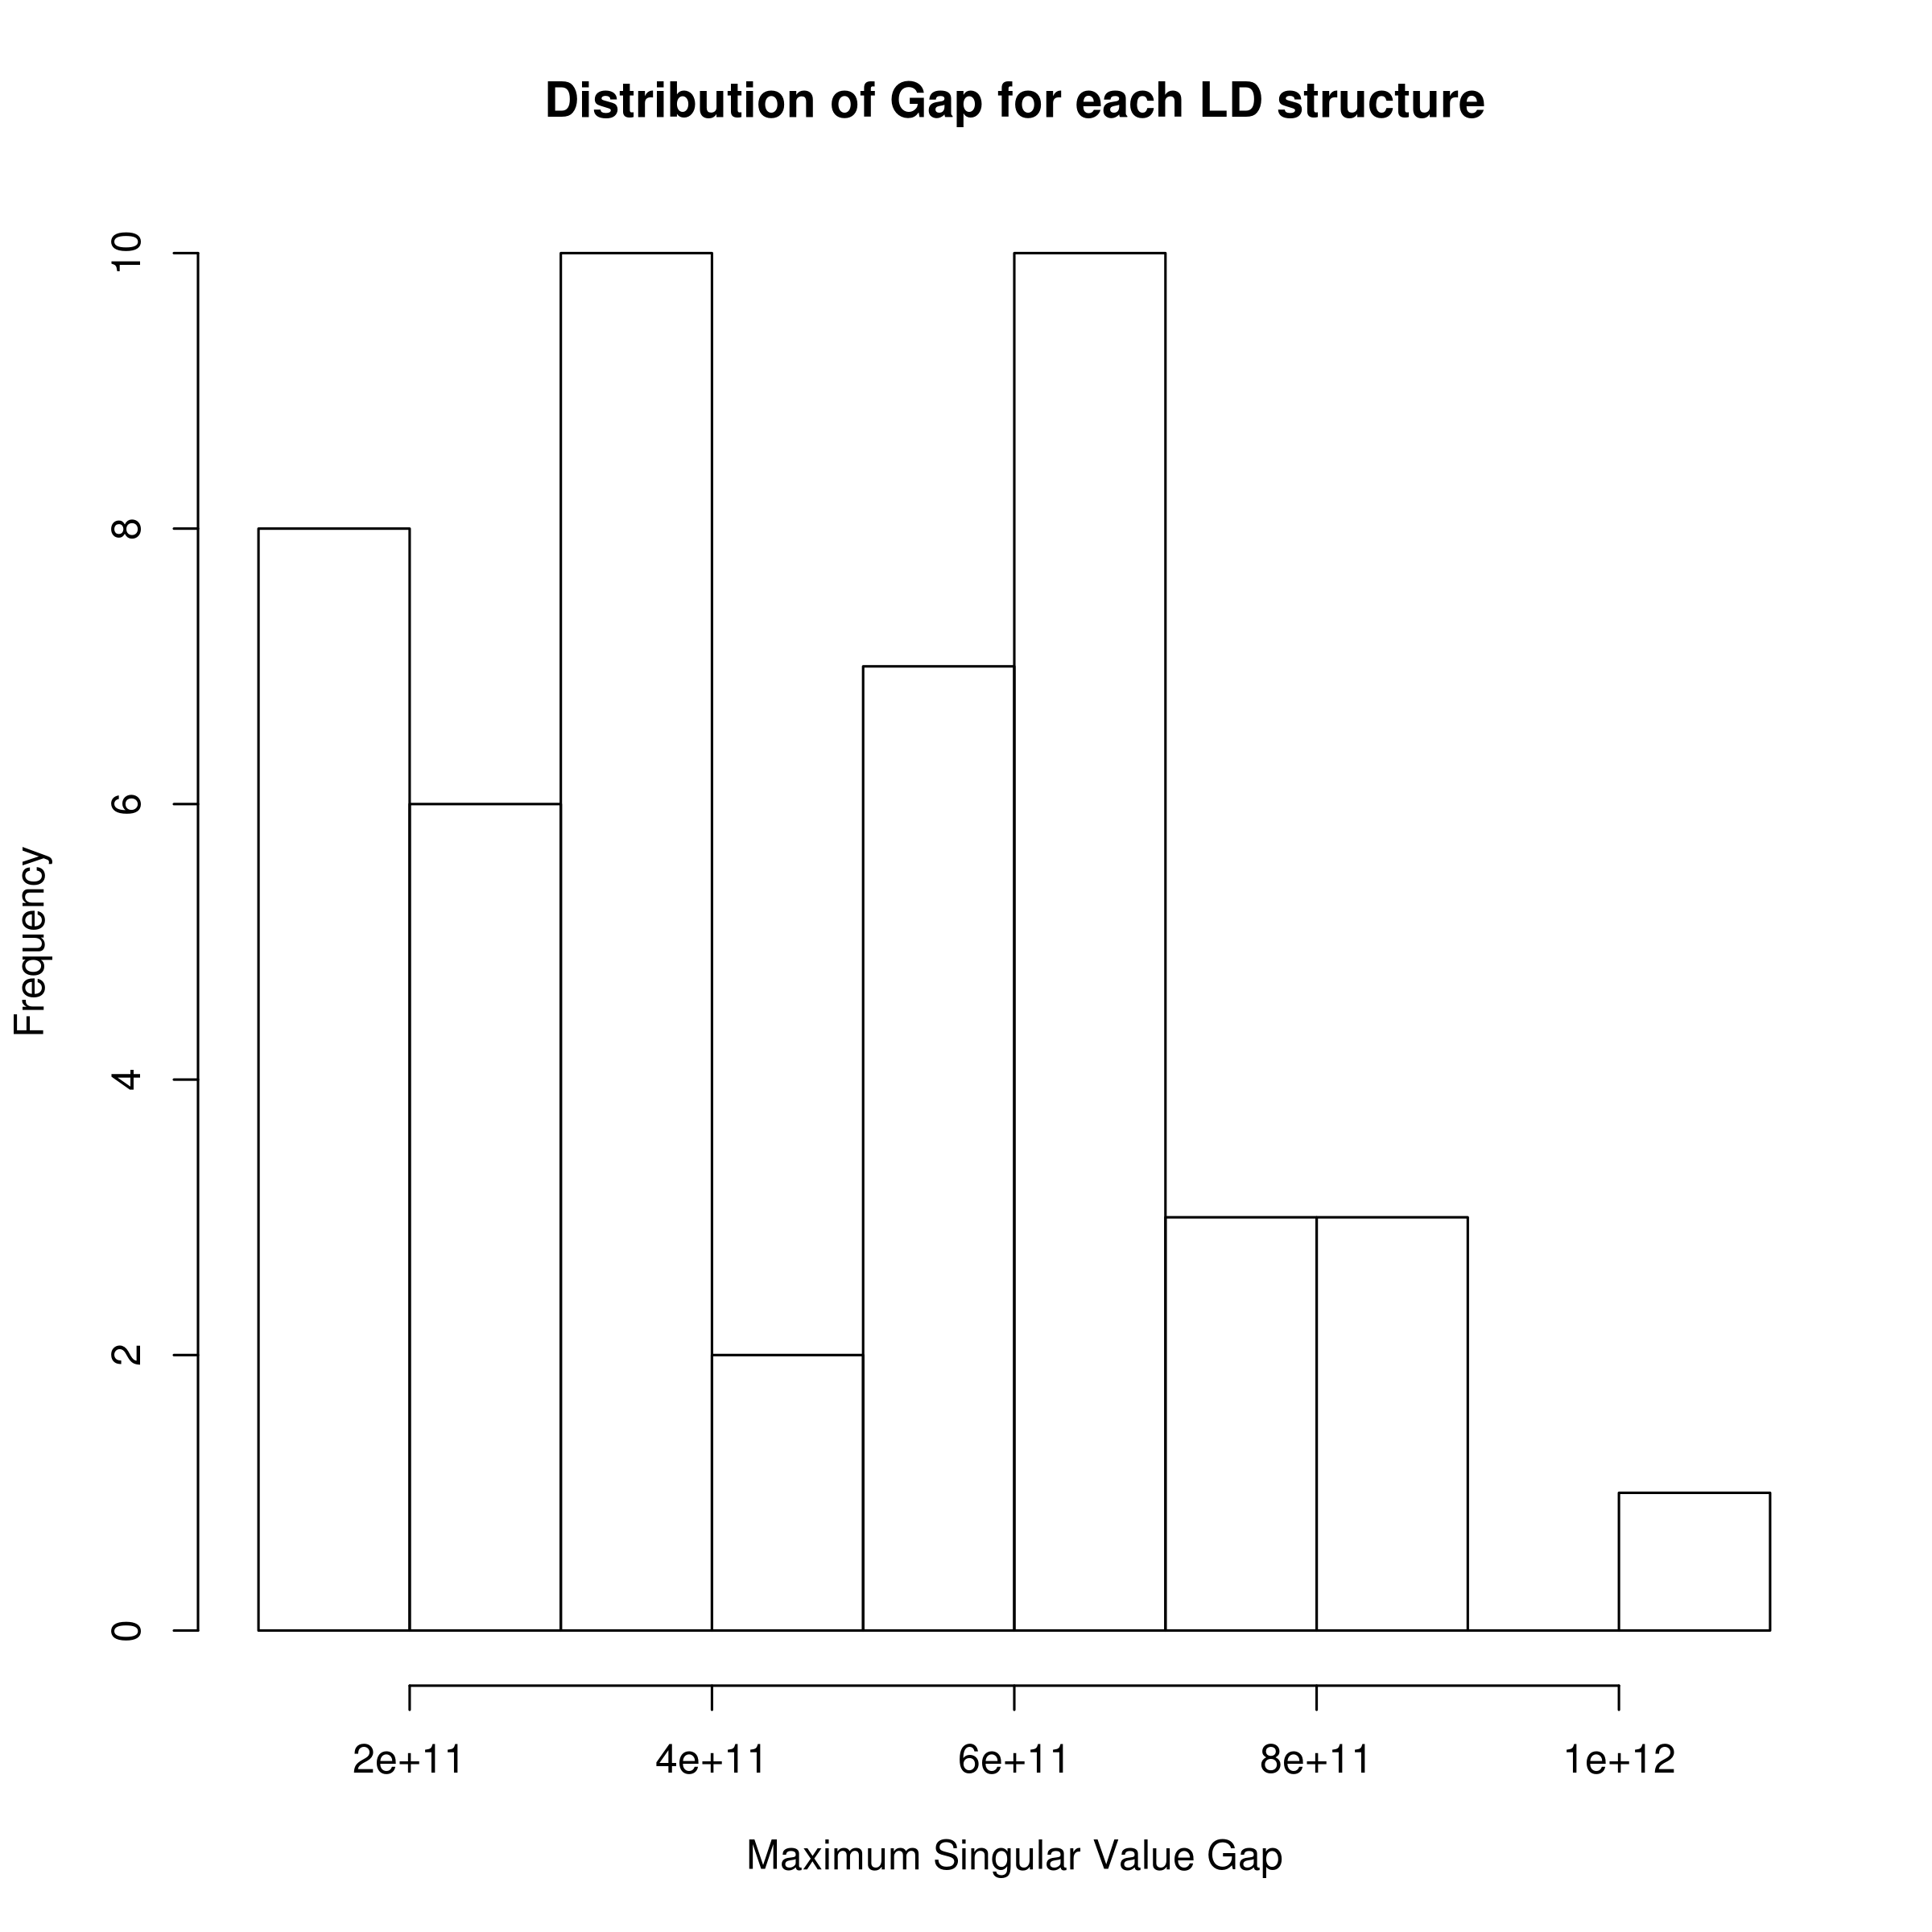
\includegraphics[width=0.5\textwidth]{figure/singular_value_distribution.png}
				\label{fig:singularValueDist}
			\end{figure}
			
			By employing the \gls{tSVD} as a method for regularization, we were able to solve the ill-posed \cref{eq:shrekEq}, and obtain the estimated heritability.
						
		\subsection{Comparing with \glsentrylong{ldsc}}
	
		
	\section{Simulation}
		We implemented the heritability estimation in \gls{shrek} and in order to assess how well \gls{shrek} performs for heritability estimation in comparison to other current methods, we performed a series of systematic simulations.
		In these simulations, we compared the performance of \gls{shrek} with \gls{gcta}\citep{Yang2011} and the \gls{ldsc}\citep{Bulik-Sullivan2015} with and without the intercept estimation function (-{}-no-intercept). 
		
		Through simulation, we can obtain the sample distribution of the heritability estimate under different study designs (e.g. Quantitativat traits, Case-Control studies or extreme phenotype selection). 
		We can also evaluate the performance of different methods under varying genetic architecture (e.g. different number of Snps, different LD structures) or even with different disease models (e.g. different number of causal Snps, different heritability).
		
		\subsection{Quantitative Trait}
			One important factor to consider when carrying out a simulation is that the result of the simulation should be translatable to real life situation. 
			Therefore, it is vital for us to consider as many different scenario as possible.
			When simulating a quantitative trait, there are a number of parameter for one to consider, for example, the sample size, the number of \glspl{SNP}, the number of causal \glspl{SNP} and the true heritability of the trait are all important parameters. 
			However, it is also unrealistic for one to test the combination of all of these parameter as that will require a large amount of processing time. 
			Thus, we aim to strike for a balance between comprehensive test case and a realistic simulation time. 
			
			First, although the average samples size for all current \gls{GWAS} was $\sim$ 7,200 samples based on \gls{GWAS} in the \gls{GWAS} Catalog\citep{Welter2014}, we only used 1,000 samples in our simulation.
			We argue that if the tools were able to perform well when a small sample size were provided, then they should perform equally, if not better, when a larger sample size is given. 
			
			Secondly, we try to capture the complex \gls{LD} structure in human population in our simulation.
			Therefore, we used HAPGEN2\citep{Su2011} with the 1000 genome \gls{CEU} population structure as an input to simulate samples with \gls{LD} structure comparable to that in the 1000 genome \gls{CEU} samples.
			Considering that it is unlikely for any \glspl{SNP} between two chromosome to be in \gls{LD}, we limit our simulation to chromosome 1 where there are a total of 670,052 \glspl{SNP} information available for use in simulation.
			However, it is noted that as number of \glspl{SNP} increase, the time required for simulating the samples and sample phenotype become prohibitive high. 
			As a result of that, we limit the number of \glspl{SNP} simulated to 50,000. 
			
			Trait complexity and trait heritability usually dictates the performance of heritability estimation.
			For example, if the trait is a Mendelian trait where there is a single causal \gls{SNP} with large effect size, it will be relatively easy to calculate the trait's heritability.
			However, when a trait is polygenic with large amount of causal \glspl{SNP}, each contribute a small portion of effect (e.g. schizophrenia), it will be challenging to estimate the heritability.
			We therefore varies the number of causal \glspl{SNP} $k$ with $k\in\{10,50,100,1000\}$ such that different spectrum of trait complexity (e.g. oligogenic to polygenic) will be tested. 
			One exception is Mendelian traits where we omit from our simulation.
			It is because Mendelian traits usually associate with a single rare \gls{SNP} with large effect size and high penetrance where its heritability can easily be estimated without the use of such complex algorithms.
			
			Besides trait complexity, the trait heritability also dictates the performance of heritability estimation. 
			We would therefore want to simulate traits with heritability $H$ where $H\in[0,1)$. 
			Based on the work of \citet{Orr1998}, we model our per-\gls{SNP} effect size to follow an exponential distribution with $\lambda=1$, which serves as a heuristic expectation of the genetic architecture of adaptation.
			Taking into account of the number of causal \glspl{SNP} and target heritability $H$, we can then calculate the per-\gls{SNP} effect size as
			\begin{align}
			\beta_i &\sim exp(1)\notag\\
			\boldsymbol{\beta}&=(\beta_1,\beta_2,...,\beta_k)^t\notag\\
			\boldsymbol{\gamma} &= \frac{H}{k}\boldsymbol{\beta}
			\label{eq:snpEffect}
			\end{align}
			where $\boldsymbol{\gamma}$ is the vector of per SNP effect size and $H$ is the simulated heritability.
			The final heritability of the simulated trait is defined as $H_{final}=\boldsymbol{1}^t\boldsymbol{\gamma}$
			
			Another consideration is the \gls{SNP} \gls{maf}, which tends to correlate with effect size\citep{Manolio2009} due to selection.
			Rare \glspl{SNP} with a small \gls{maf} tends to have a large effect size whereas common \glspl{SNP} tends to have a small effect size. 
			Therefore, after the per \gls{SNP} effects were simulated, we distribute the effect size to $k$ randomly selected \gls{SNP}(s) according to their \gls{maf}.
		
			Finally, by assuming $\boldsymbol{X}$ to be the standardized genotype of $k$ causal SNPs in $n$ samples, one can get the phenotype of the simulated samples based on \cref{eq:snpEffect} using
			\begin{align}
			\epsilon_i&\sim N(0,\sqrt{\mathrm{Var}(\boldsymbol{X\gamma})\frac{1-H_{final}}{H_{final}}} )\notag\\
			\boldsymbol{\epsilon} &= (\epsilon_1,\epsilon_2,...,\epsilon_n)^t\notag\\
			\boldsymbol{y} &= \boldsymbol{X\gamma}+\boldsymbol{\epsilon}
			\label{eq:simulationOfPhenotype}
			\end{align}
			
			For each batch of simulated samples, we calculate the estimated heritability using \gls{shrek}, \gls{gcta}, \gls{ldsc} without intercept estimation and \gls{ldsc} with intercept estimate (\textit{\texorpdfstring{LDSC\textsubscript{In}}}) for each $H$.
			In each iteration, the sample genotype was provided to \gls{gcta} for the calculation of genetic relationship matrix (GRM) whereas for \gls{shrek} and \gls{ldsc} 500 additional samples were simulated based on the 1000 genome project \gls{CEU} samples\parencite{Project2012} to construct the \gls{LD} matrix and calculate the \gls{LD} score respectively. 
			This is because in general situations, \gls{ldsc} and \gls{shrek} will not be provide with the sample genotype, instead, these programmes were designed to work with external \gls{LD} reference data.
			Therefore to provide a realistic simulation, an independent set of reference samples were provided for \gls{shrek} and \gls{ldsc}.
			  
			The whole process were repeated 100 times to obtain the empirical variance of the estimates,.
			In each iteration, new set of samples were simulated with the \glspl{SNP} set, the causal \glspl{SNP} and the per \gls{SNP} effect size remain unchanged for each $H$.
			%In order to determine a realistic and reasonable sample size for all simulation condition, we manually curated the sample size of all the studies presented on the \gls{GWAS} Catalog\cite{Welter2014} (version 2015-07-17) to get the distribution of sample size in existing studies.
			%It was observed that the mean sample size of all published \gls{GWAS} is $\sim$ 7,200 samples. 
			%Thus, we consider a simulation sample size of 7,200 should be comparable to general \gls{GWAS} studies.
			%Although a large sample size are generally required for \gls{GWAS}, it might also worthwhile for one to test the performance when only small sample size is available.
			%If the tools perform well with a small sample size, it will be beneficial to studies of rare complex traits where it is often difficult to collect a large amount of samples.
			%As a result of that, we also perform simulation with 1,000 samples.
			
			To summarize, 
			\begin{enumerate}
				\item Randomly select 50,000 \glspl{SNP} from chromosome 1
				\item Randomly generate $k$ effect size following \cref{eq:snpEffect} where $k \in \{10,50,100,1000\}$
				\item Randomly assign the effect size to $k$ \glspl{SNP} where \glspl{SNP} with small \gls{maf} will get a large effect size.
				\item Simulate 1,000 samples using \textit{HAPGEN2} and calculate their phenotype according to \cref{eq:simulationOfPhenotype}
				\item Repeat step 4 100 times
				\item Repeat step 1-5 50 times
			\end{enumerate}
			
			
		\subsection{Case Control Studies}
		Simulate of the case control studies are very much like that in the quantitative trait settings except that we will have to generate the phenotype according to a liability threshold.
		
		\subsection{Exreme Phenotype Selections}
	\section{Result}
		The heritabilibty estimation were implemented in \gls{shrek} and is available on \url{https://github.com/choishingwan/shrek}.
		
	\section{Discussion}
	
	\chapter{Heritability of Schizophrenia}
	\section{Introduction}
	Apply Heritability estimation to the schizophrenia data.
	The genetic correlation and partitioning of heritability
	No one worked on linking schizophrenia with brain development directly?
	% talk about the current research on schizophrenia?
	% the overall heritablity estimation
	% The genetic correlation done by the LDSC. 
	% The theory of brain development 
	% How the co-expression network works
	% Drug response?
	\section{Heritability Estimation}
	This will be a very simple section, focused on how to perform the heritability estimation on \acrfull{SCZ}.
	Should also tokenize the heritability into subcategories (e.g. immune, neuron, etc)
	%Should not put too much weight into it, otherwise it will be a direct copy of LDSC. Won't really add much power. 
	
	
	\subsection{Methodology}
	\subsection{Result}
	\section{Brain development and Schizophrenia}
	\sectionmark{Brain development}
	Here we will perform the WGCNA and brain development network.
	Seeing how the whether if any brain development network were enriched with SNPs that explain the variance of phenotype
	%Instead, we should put most focus here as no one has done it before
	%Also descript brainspan here
	\subsection{Methodology}
	\subsubsection{Sample Quality Controls}
	We obtain the developmental transcriptome data from BrainSpan (\url{http://www.brainspan.org/}). 
	A total of 56 samples with different age were provided by BrainSpan with an average of 2.2 samples per age.
	
	Studies suggested Hippocampus\citep{Velakoulis2006,Nugent2007}, Amygdala and Striatum\citep{Simpson2010} are brain regions involved in the etiology of schizophrenia. 
	Therefore, we focus on building the gene co-expression network of hippocampus, amygdala and striatum in this study
	It is worth noting that the Pre-frontal Cortex is also important for schizophrenia. 
	However, as there isn't a well defined pre-frontal cortex samples from BrainSpan, we did not include the pre-frontal cortex in the current study.
	RNA Sequencing data of the brain regions were obtained from BrainSpan and undergo a series of quality control before the construction of the network. 
	 
	For each sample age, when there are more than one samples, we select the sample with a dissection score $\ge3$ and an \gls{rin} $\ge7$. 
	As some developmental stage only got 1 sample passing the quality check, we limit each developmental stage to have a maximum of 1 sample such that the final network will not be driven by a particular developmental stage. 
	If multiple samples passed through the quality check threshold, we will prefer sample with higher dissection score. 
	Shall multiple samples have the same dissection score, we will select the one with the highest \gls{rin}. 
	And if the samples have the same dissection score and \gls{rin} value, we will randomly select one for the network construction.
	
	After performing the quality control, a total of 16, 18 and 15 samples were selected for hippocampus, amygdala and striatum respectively.
	The sample age ranged from \gls{gd}8 to 23 years old representing the fetal developmental stage till the age of onset of schizophrenia.
	
	\subsubsection{Normalization of data}
	The RNA Sequencing data were represented as \gls{rpkm} values. 
	Genes with a low \gls{rpkm} can usually be a result from technical or biological noise\citep{Hart2013}.
	To reduce noise in the final model, genes with a mean \gls{rpkm} $< 1$ in all samples were discarded. 
	The \gls{rpkm} were then log transformed as instructed by the manual of \gls{wgcna}\citep{Langfelder2008}.
	
	As there are insufficient samples for the construction of gene co-expression network for individual sample age, we try to construct networks with genes co-expressed through all sample stage. 
	This is achieved by taking the standardized log$_2$ \gls{rpkm} across sample age such that all genes has a mean of 0 and standard deviation of 1.
	
	At the end, there were 17,168 genes, 17,038 genes and 17,166 genes passing through the quality threshold and were used for the construction of co-expression network in hippocampus, amygdala and striatum respectively. 
	 
	\subsubsection{Network Construction}
	\gls{wgcna} (ver 1.47) were used for the construction of gene co-expression network\citep{Langfelder2008}. 
	The \emph{blockwiseModules} function, using Biweight Midcorrelation for the construction of correlation matrix and a restriction of minimum network size of 30. 
	For the construction of gene co-expression networks in hippocampus, the soft-power threshold were set to 15 where it is the first threshold value which has $R^2 > 0.8$ (0.817) and the $R^2$ is saturated\citep{Zhang2005}.%(\cref{fig:softpowerThreshold})
	As for striatum, the soft-power threshold were set to 20. 
	Again, this is the first threshold value with $R^2 >0.8$ (0.879) and where the $R^2$ is saturated.
	
	On the other hand, for amygdala, soft-power threshold were set to 9 which is the first threshold for $R^2$ to reach saturation. 
	However, with a soft-power threshold of 9, the $R^2$ were only 0.776, which is lower than the recommended 0.8 threshold.
	The reason behind this decision was that the first soft-power threshold to have $R^2 > 0.8$ is 30.
	Under this threshold, the mean connectivity of the resulting networks will be around 23.6 with a median connectivity of 2.51.
	Such level of connectivity will likely yield networks that are too small to useful.
	If one would like to satisfy both requirement of threshold selection, a threshold $>30$ are likely required and any networks constructed will likely to be small.
	As a result of that, we select threshold of 9 where networks with reasonable size can be constructed.
	
	%\begin{figure}
	%	\caption[Soft-power threshold selection]{Soft-power threshold selection. A soft-power of 13 were selected as it is the first threshold value having $R^2 > 0.8$ (0.817) and where the $R^2$ is saturated.}
	%	\centering
	%	\scalebox{.8}{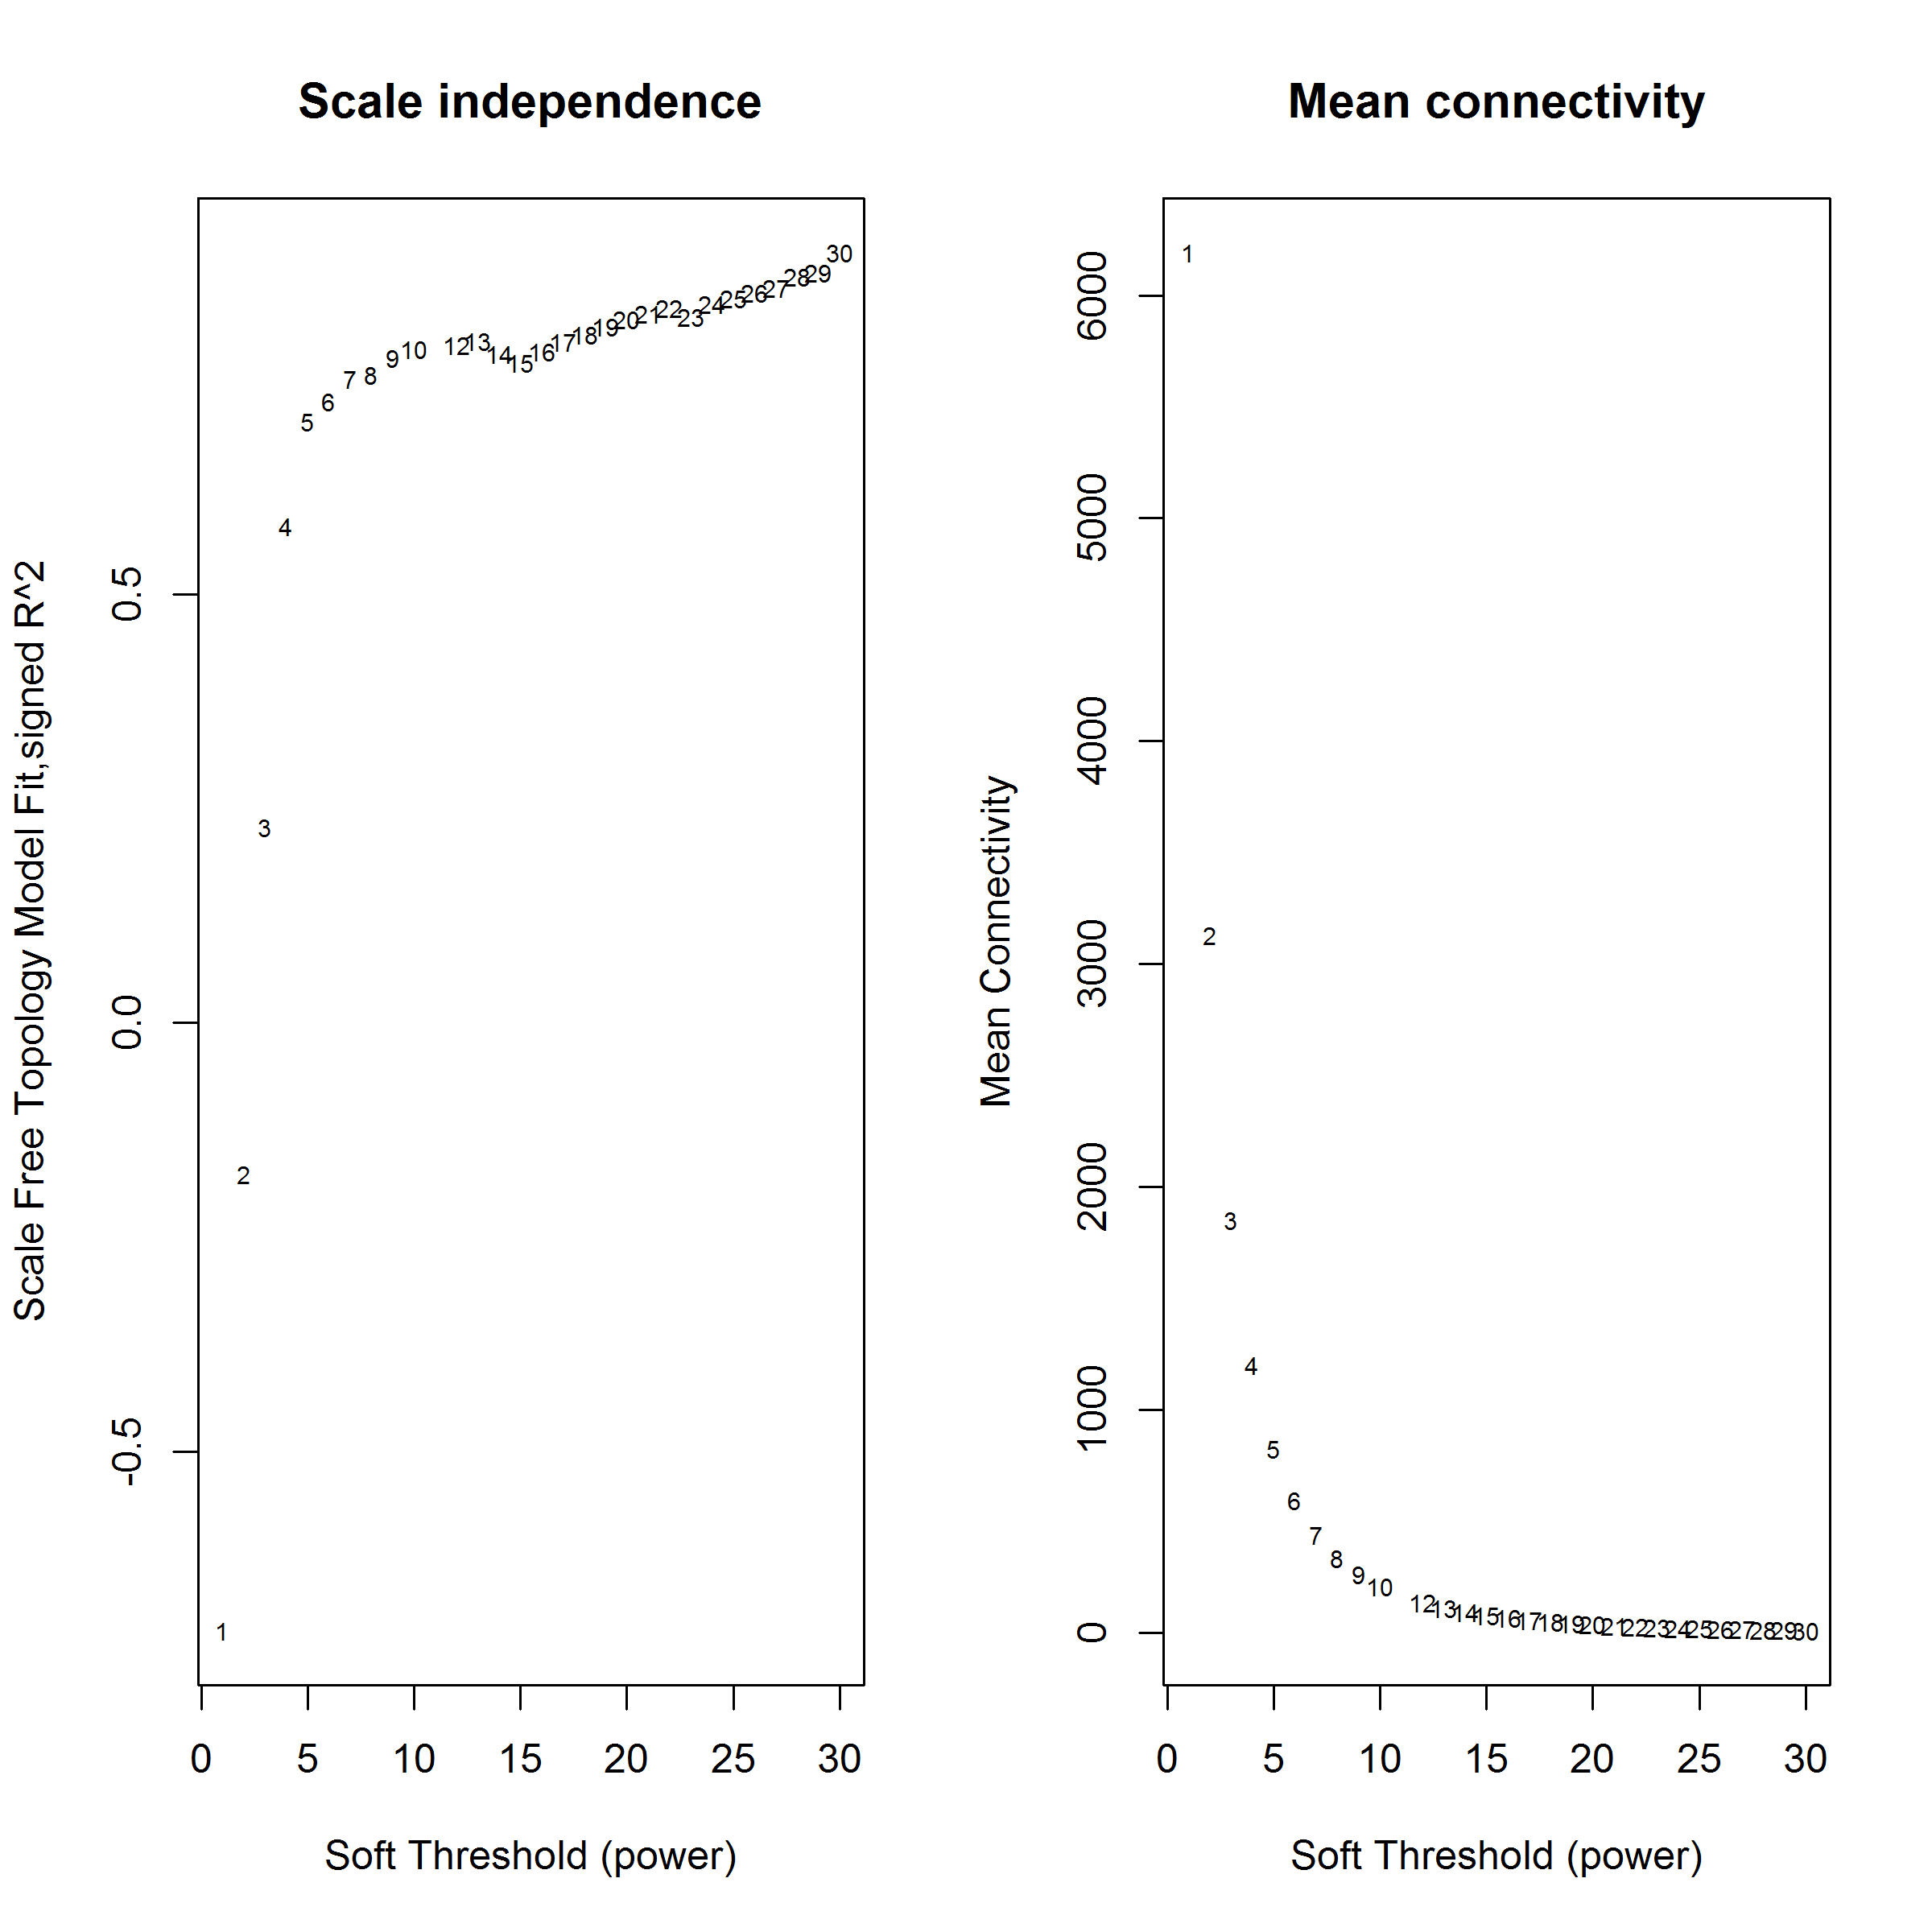
\includegraphics{figure/SoftpowerThreshold.png}}
	%	\label{fig:softpowerThreshold}
	%\end{figure}
	
	\subsubsection{Expression correlation with Age}
	The co-expression network constructed with the standardized gene expression value will contains genes that co-express in all sample age.
	However, this does not necessary suggest the expression of these genes are correlated with the sample age.
	To identify gene co-expression networks with expressions correlated with the sample age, we performed a correlation analysis between the module eigen-genes and the sample age. 
	Network eigen-genes were calculated as the first \gls{pc} of expressions of the genes within individual networks using the \emph{moduleEigengenes} function from \gls{wgcna}. 
	Age were represented as month from conception such that 8 post-conception week will be represented as 2; 4 months will be represented as 10 and 12 years will be represented as 154 etc. 
	Finally, correlation between age and network eigen-gene expression were calculated pearson correlation.
	
	\subsubsection{Functional Annotation}
	\gls{GO} based enrichment analysis of the significant module was performed using GOrilla\citep{Eden2009}.
	Genes within the networks were provide as the target gene lists and all the genes passed quality controls were used as the background gene list.
	As \gls{GO} terms tends to be redundant and overlaps with each other, it will aid the interpretation of \gls{GO} results based by clustering and reducing the \gls{GO} terms based on their similarity. 
	Thus, \gls{GO} enrichment results were summerized by REViGO\citep{Supek2011} and significant representative \gls{GO} terms were obtained.
	
	\subsubsection{Associate Co-expression network with \glsentryshort{pgc} schizophrenia data}
	The co-expression networks were built from normal samples and should not be representative of the brain expression pattern in schizophrenia patients.
	it is however interesting to see if the co-expression networks were disrupted in schizophrenia patient.
	To test whether if the gene co-expression networks contain genes that are jointly associated with schizophrenia, we first use \gls{MAGMA}\citep{DeLeeuw2015}(version v1.03) to compute the gene-base p-value from the \gls{SNP} wise p-value obtained from \gls{pgc}. 
	Gene-set enrichment analysis were then performed on networks that were significantly correlated with developmental age. 
	As we were only interested in whether if the genes within the networks were jointly associated with schizophrenia, we only focus on the result of the self-contained gene set analysis and ignore the result from competitive analysis.
	
	\subsubsection{Partitioning of Heritability}
	
	\subsection{Result}
	\subsubsection{Co-Expression Network}
	A total of 35 networks were constructed based on the hippocampus samples with a mean network size of 421.6.
	On the other hand, 28 networks were constructed for amygdala with mean network size of 591.86.
	Finally, 25 networks with mean size of 494.52 were constructed from the striatum samples.
	
	Of the all the networks constructed, only one network from hippocampus(\cref{tab:hipModSig}) and three networks from amygdala(\cref{tab:amyModSig}) were significantly correlated with sample age after bonferroni correction threshold (p-value $<0.00143$ for hippocampus, p-value $<0.00179$ for amygdala and p-value $<0.002$ for striatum) .
	\begin{table}
		\centering
		\caption[Correlation of sample age with the module eigen gene]{Correlation of sample age with the module eigen gene. 
			Module eigen-gene was defined as the first \gls{pc} of genes within the module. 
			After correcting for multiple testing, only the black module was considered as significantly correlated with the sample age.}
		\subfloat[Hippocampus]{
			\begin{tabular}{rrr}
				\toprule
				& Correlation & Pvalue \\
				\midrule
				black & 0.804653 & 0.000171 \\
				blue  & -0.61648 & 0.010981 \\
				red   & -0.60207 & 0.013595 \\
				darkred & -0.59137 & 0.015833 \\
				greenyellow & -0.56995 & 0.021168 \\
				yellow & 0.567828 & 0.021763 \\
				darkgrey & -0.55246 & 0.026474 \\
				saddlebrown & -0.52983 & 0.034783 \\
				turquoise & -0.51371 & 0.041809 \\
				purple & -0.46788 & 0.067606 \\
				darkolivegreen & -0.41272 & 0.112122 \\
				sienna3 & -0.39535 & 0.129604 \\
				darkturquoise & 0.386541 & 0.139154 \\
				darkorange & 0.384966 & 0.140912 \\
				darkmagenta & 0.375586 & 0.151688 \\
				brown & 0.366095 & 0.163144 \\
				tan   & -0.36522 & 0.164229 \\
				pink  & 0.348979 & 0.18524 \\
				magenta & -0.32559 & 0.218473 \\
				midnightblue & -0.29168 & 0.273014 \\
				lightgreen & 0.289921 & 0.276056 \\
				paleturquoise & -0.28045 & 0.29276 \\
				white & 0.27727 & 0.29849 \\
				orange & 0.19607 & 0.466754 \\
				steelblue & 0.17355 & 0.520357 \\
				skyblue & 0.145869 & 0.589857 \\
				lightyellow & -0.11665 & 0.667028 \\
				green & -0.09882 & 0.715786 \\
				violet & -0.08757 & 0.747076 \\
				lightcyan & -0.0656 & 0.809257 \\
				cyan  & -0.06441 & 0.812661 \\
				darkgreen & -0.03914 & 0.885582 \\
				salmon & 0.038727 & 0.886769 \\
				royalblue & -0.03785 & 0.889314 \\
				grey60 & 0.03119 & 0.908709 \\
				\bottomrule
				\label{tab:hipModSig}%
			\end{tabular}%
		}
		\qquad%
		\subfloat[Amygdala]{
			\begin{tabular}{rrr}
				\toprule
				& Correlation & P-value \\
				\midrule
				tan   & 0.849999 & $7.96\times 10^{-6}$ \\
				yellow & -0.757 & $2.76\times 10^{-4}$ \\
				pink  & -0.68541 & $1.69\times 10^{-3}$ \\
				greenyellow & -0.67831 & $1.97\times 10^{-3}$ \\
				red   & -0.64532 & $3.83\times 10^{-3}$ \\
				turquoise & -0.59771 & $8.80\times 10^{-3}$ \\
				lightyellow & -0.56347 & 0.0149 \\
				brown & 0.548516 & 0.0184 \\
				darkgreen & -0.46366 & 0.0526 \\
				blue  & -0.4604 & 0.0545 \\
				purple & -0.44182 & 0.0664 \\
				darkgrey & -0.39065 & 0.109 \\
				orange & -0.36966 & 0.131 \\
				white & 0.28737 & 0.248 \\
				darkred & 0.283247 & 0.255 \\
				black & 0.271383 & 0.276 \\
				salmon & -0.24203 & 0.333 \\
				skyblue & 0.207071 & 0.410 \\
				cyan  & 0.18778 & 0.456 \\
				lightgreen & 0.166495 & 0.509 \\
				grey60 & 0.15156 & 0.548 \\
				midnightblue & 0.136078 & 0.590 \\
				magenta & -0.13459 & 0.594 \\
				darkturquoise & 0.129954 & 0.607 \\
				lightcyan & 0.090241 & 0.722 \\
				darkorange & -0.05166 & 0.839 \\
				green & -0.04745 & 0.852 \\
				royalblue & 0.020456 & 0.936 \\
				\bottomrule
				\label{tab:amyModSig}%
			\end{tabular}%
		}
	\end{table}
	
	By plotting the mean expression of each network against the sample age, one can inspect how the dynamic of the network changes across different developmental stage.
	Thus, mean expression of all the genes within the significant networks were calculated for all amygdala (n=33) and hippocampus (n=32) samples from BrainSpan.
	The mean \gls{rpkm} values were then log$_2$ transformed and plot against the sample age where a line of bests fit was calculated using the \emph{stat\_smooth} with the loess function from R package \emph{ggplot2}(version 1.0.1). (\cref{fig:allMod}).
	
	The expression pattern observed were intriguing where there both the ``black''(\cref{fig:blackMod}) and ``tan'' (\cref{fig:tanMod}) networks have mean gene expression level increase as development progress and reaches its peak at around late adolescence ($\approx 18-21$), concurring with the onset age of schizophrenia.
	Similarly, an inverse pattern were observed with the ``yellow'' network where its mean expression was highest during fetal development and drop steadily to its lowest around late adolescence and increase again afterwards(\cref{fig:yellowMod}).
	
	The expression pattern of the ``black'' and ``tan'' networks are of particular interest as they follow the inverted ``U'' shape trajectory of the grey matter volumn observed in previous studies\citep{Gogtay2011}, suggest that they might have a role in mediating brain development. 
	\begin{figure}
		\caption[Mean Gene Expression across developmental age]{Mean Gene Experssion across developmental age.
			Mean \gls{rpkm} values of genes in the significant modules were plot with respect to the sample age.
			A loess smoothing curve was also plotted. 
			%Might want to talk somemore about it
		}
		\centering
		\subfloat[``Black'' Network from Hippocampus]{
			\scalebox{.4}{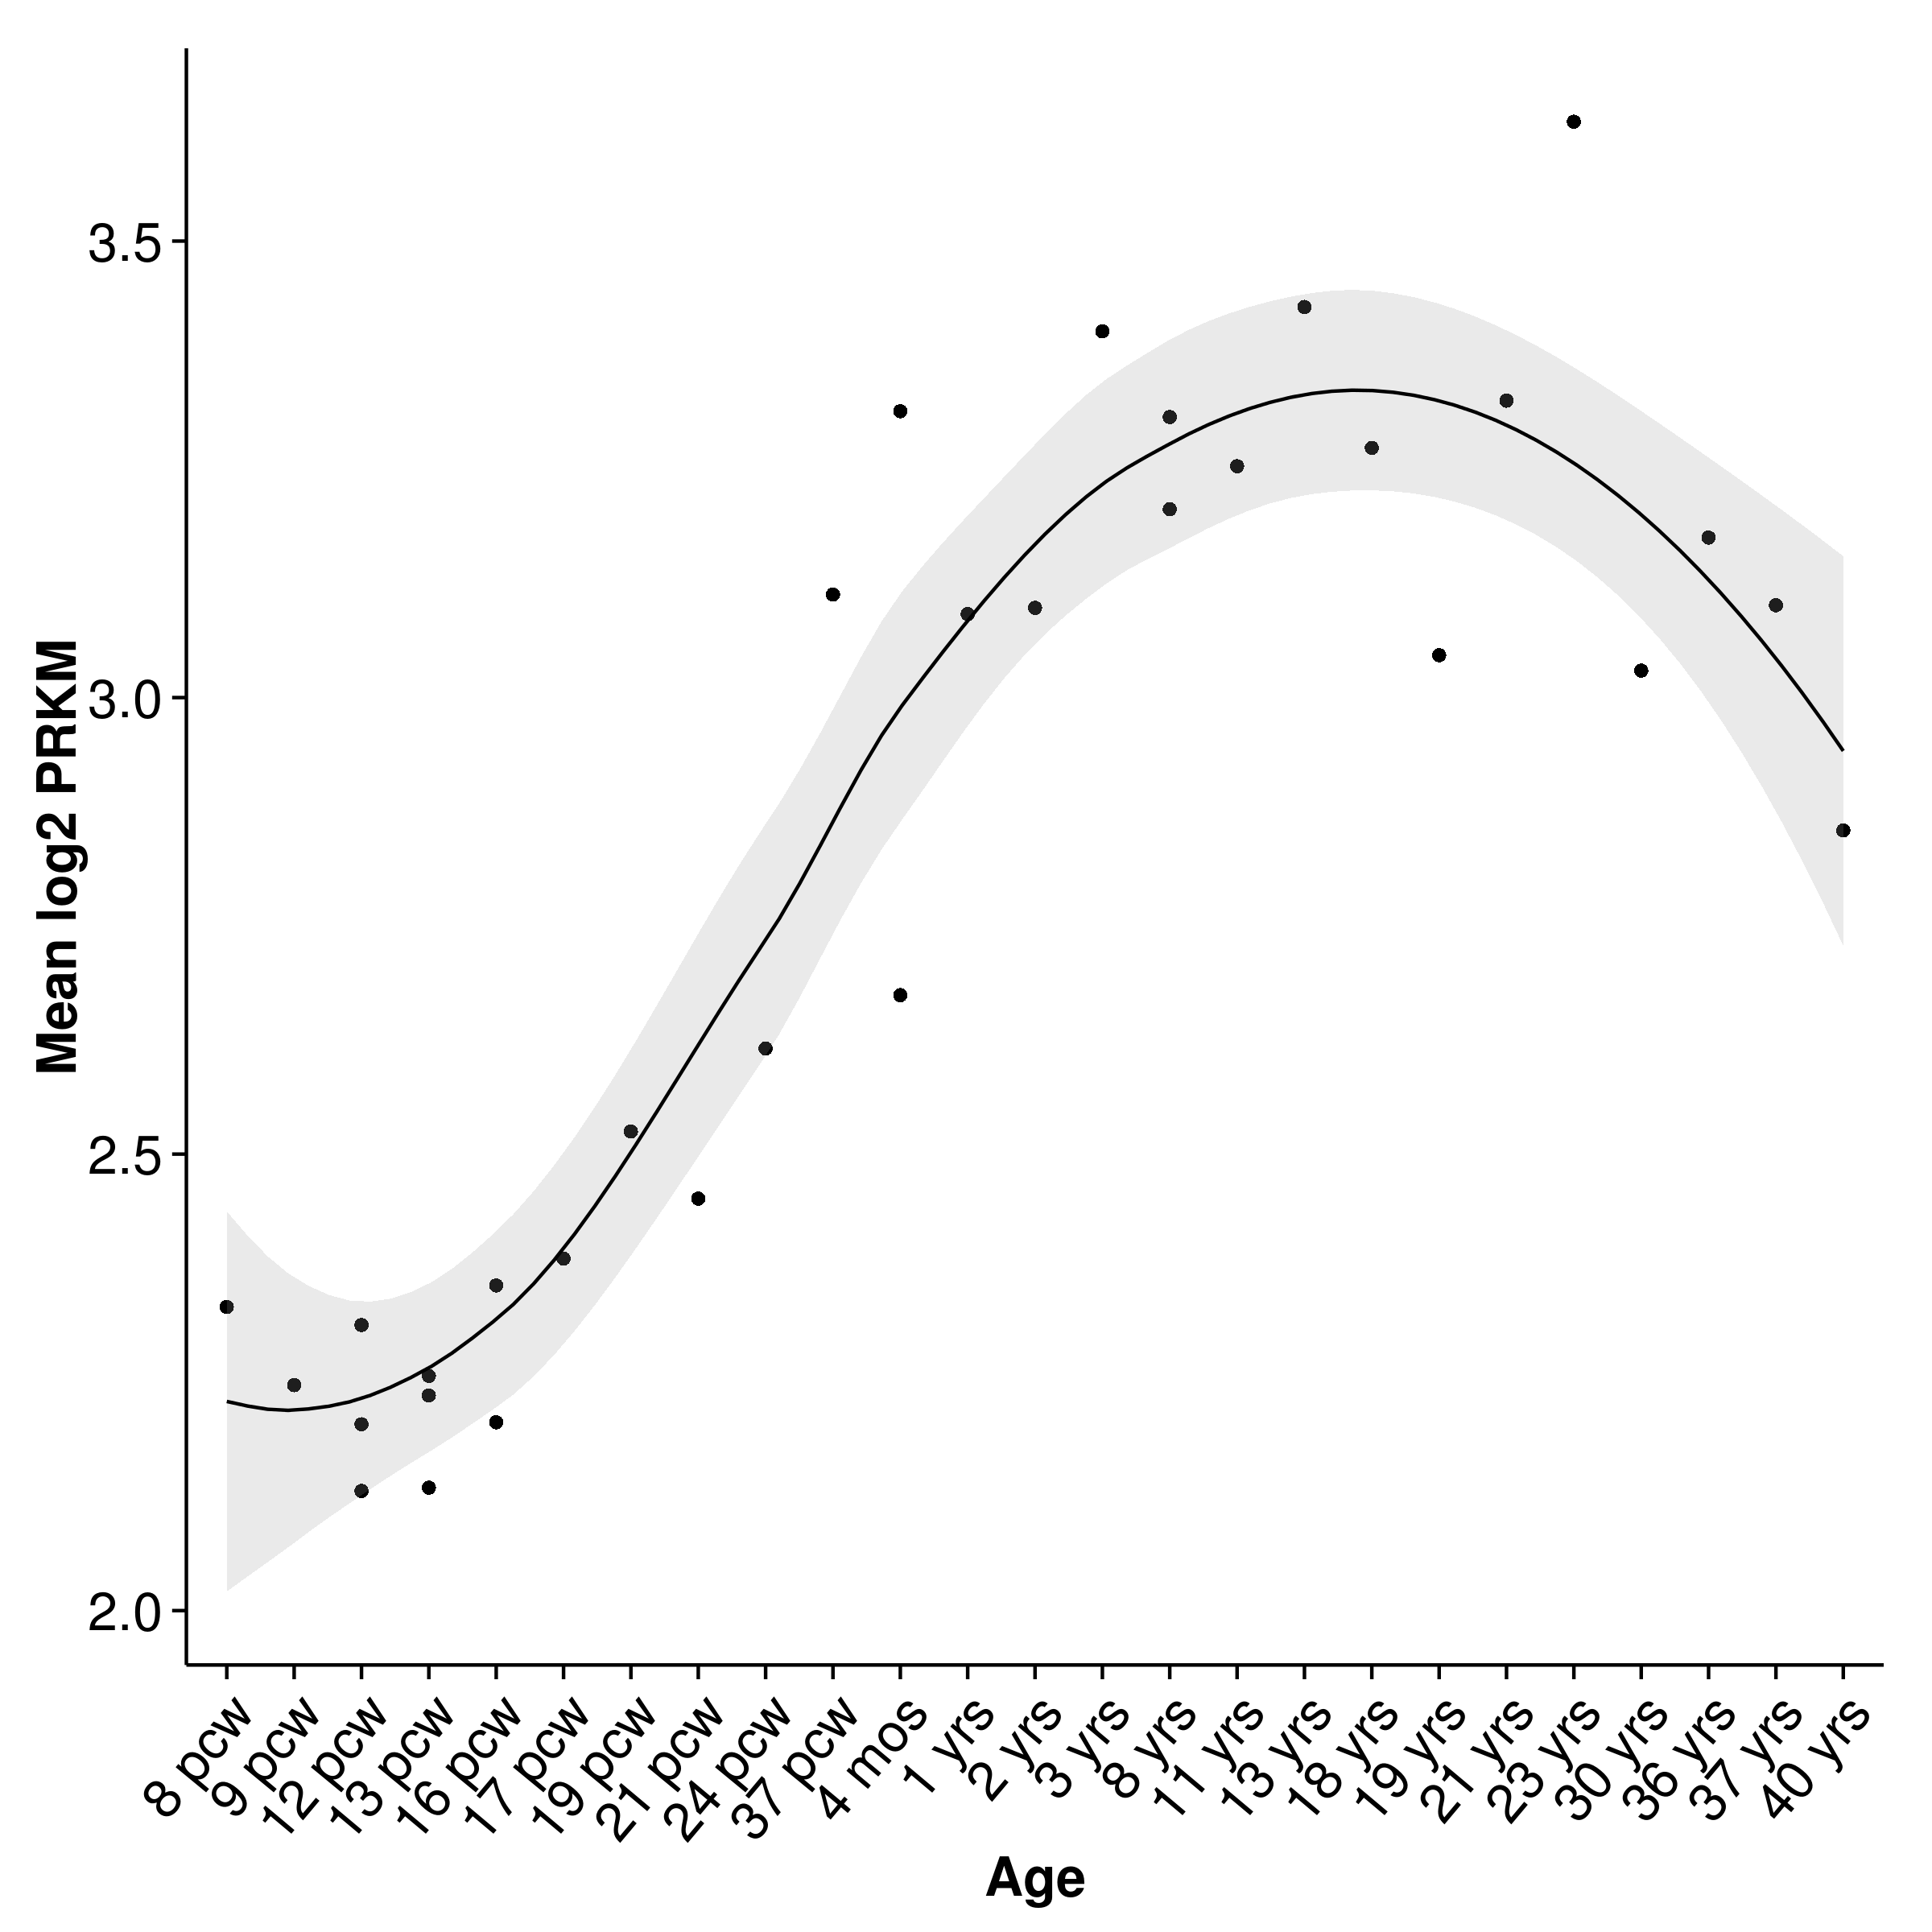
\includegraphics{figure/network/hip_network.png}}
			\label{fig:blackMod}
		}
		\subfloat[``Tan'' Network from Amygdala]{
			\scalebox{.4}{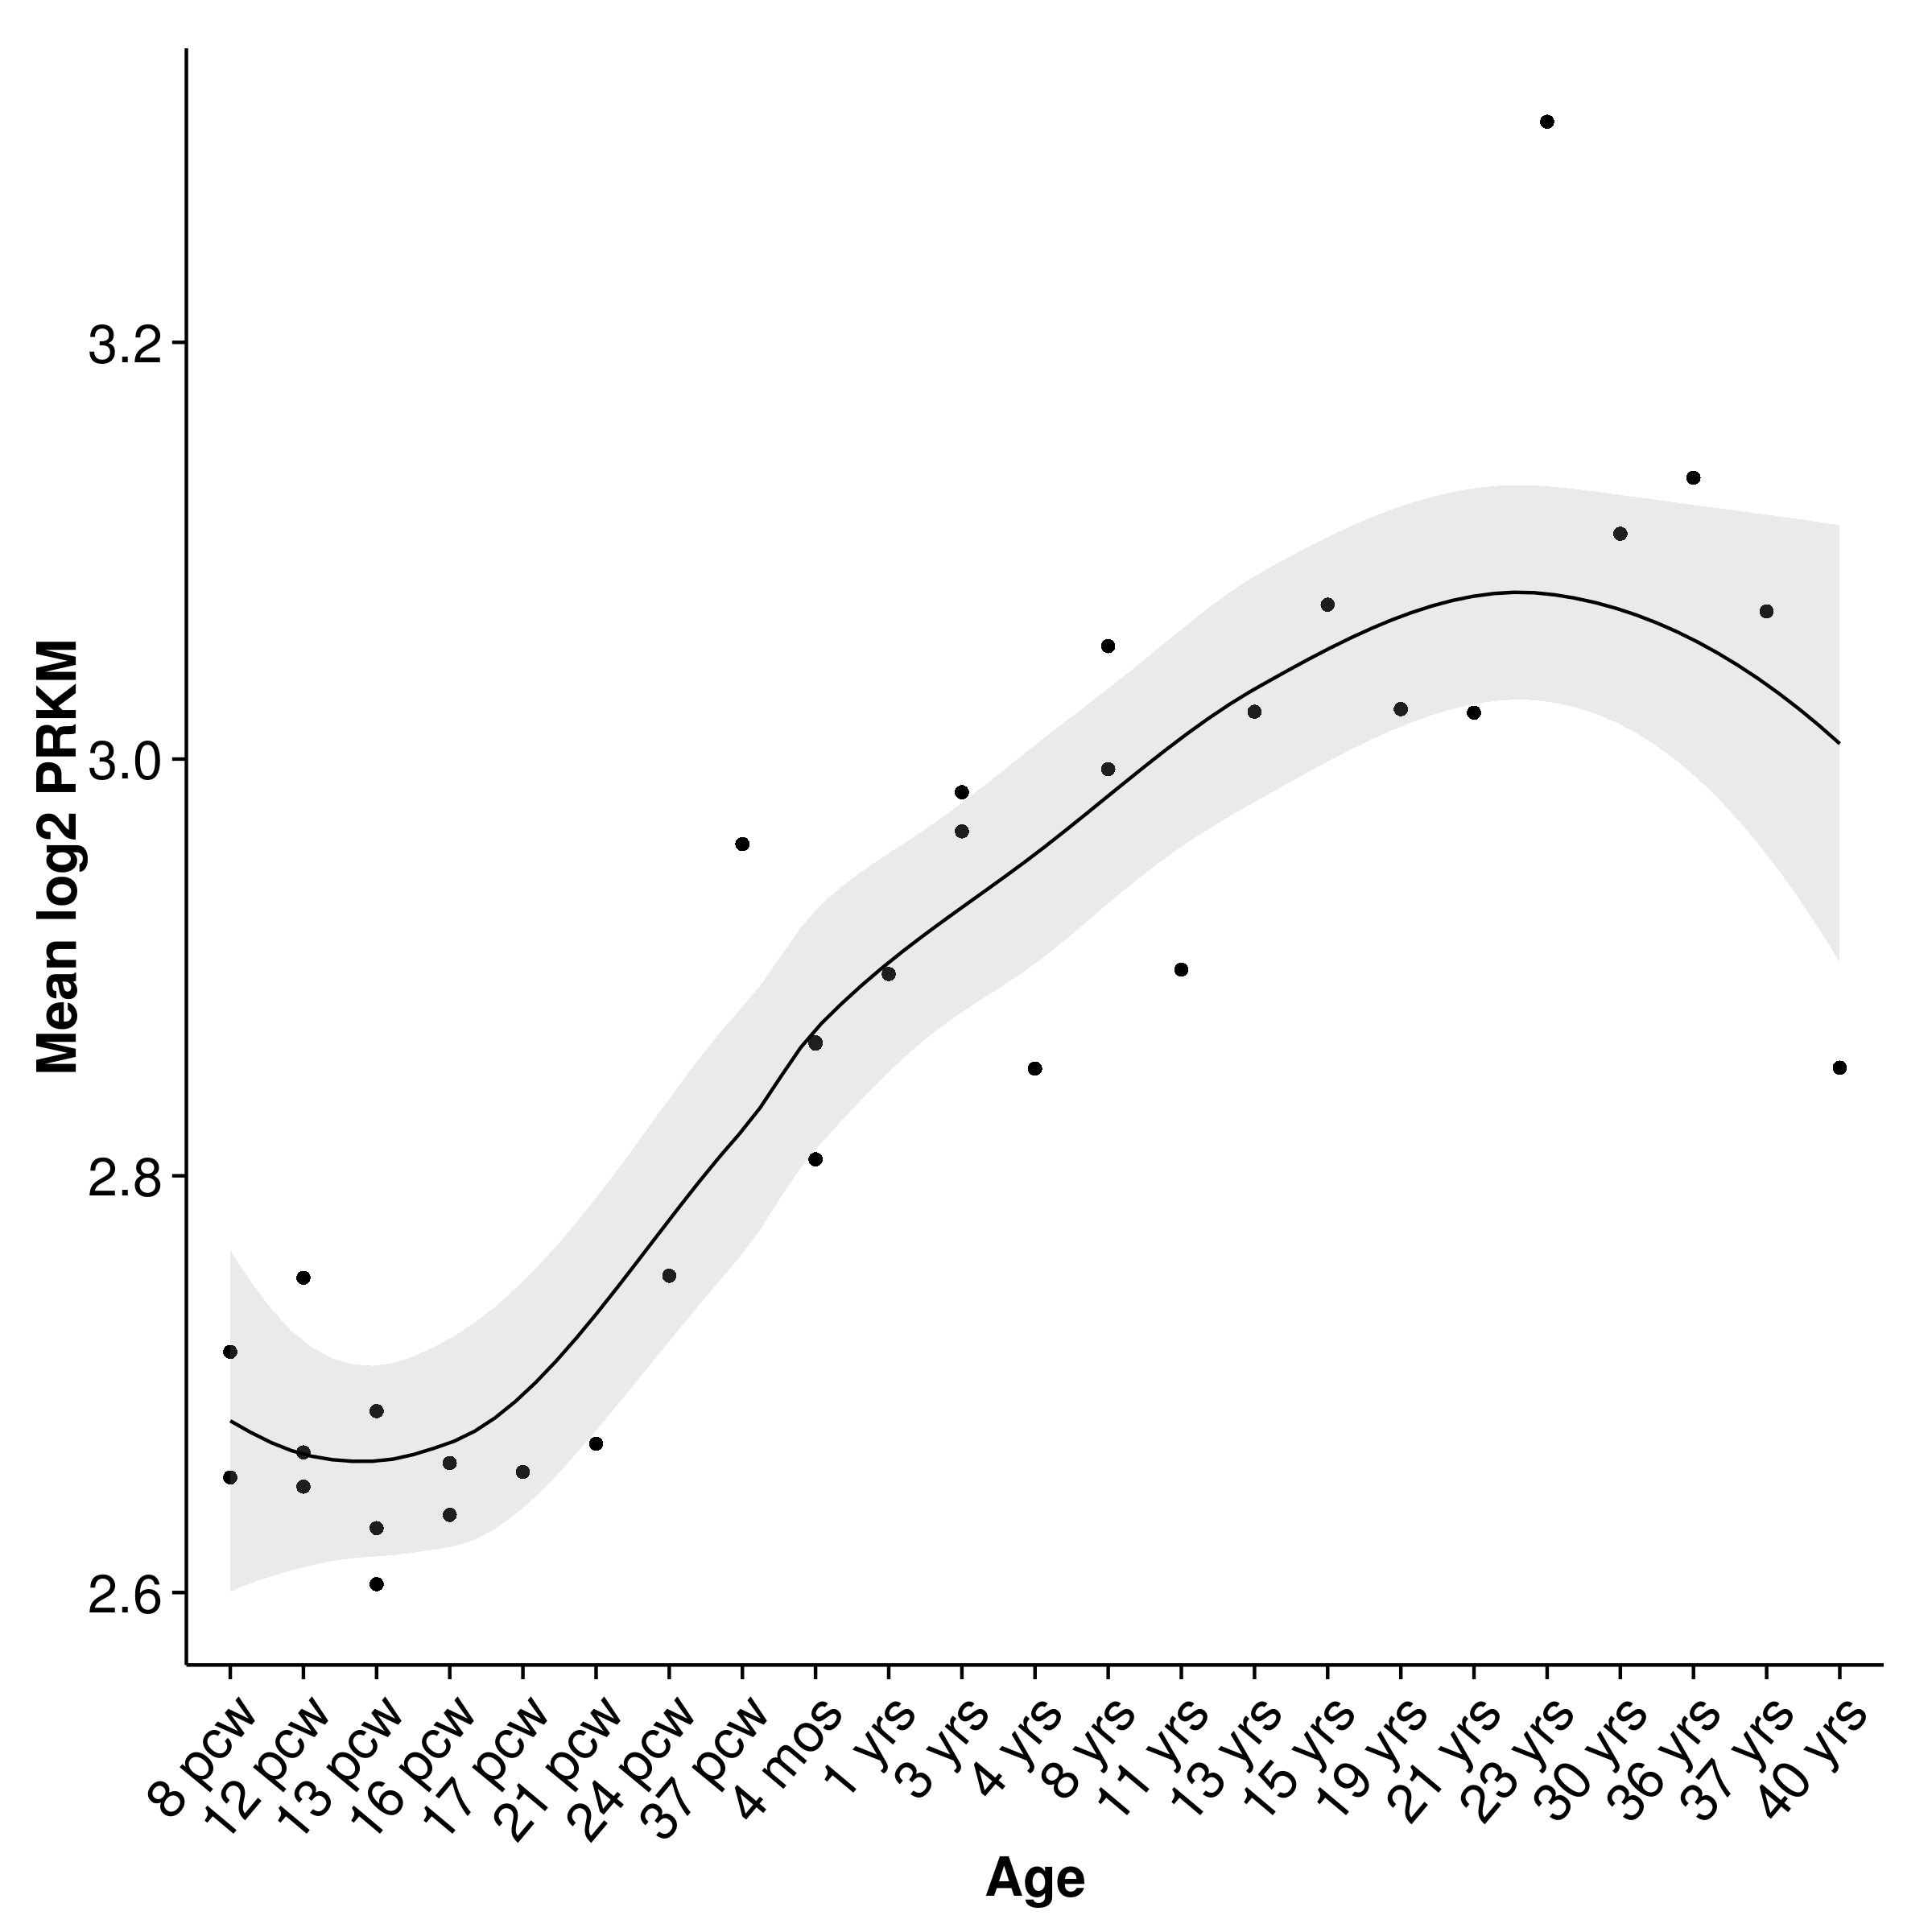
\includegraphics{figure/network/amy_tan_network}}
			\label{fig:tanMod}
		}\\
		\subfloat[``Pink'' Network from Amygdala]{
			\scalebox{.4}{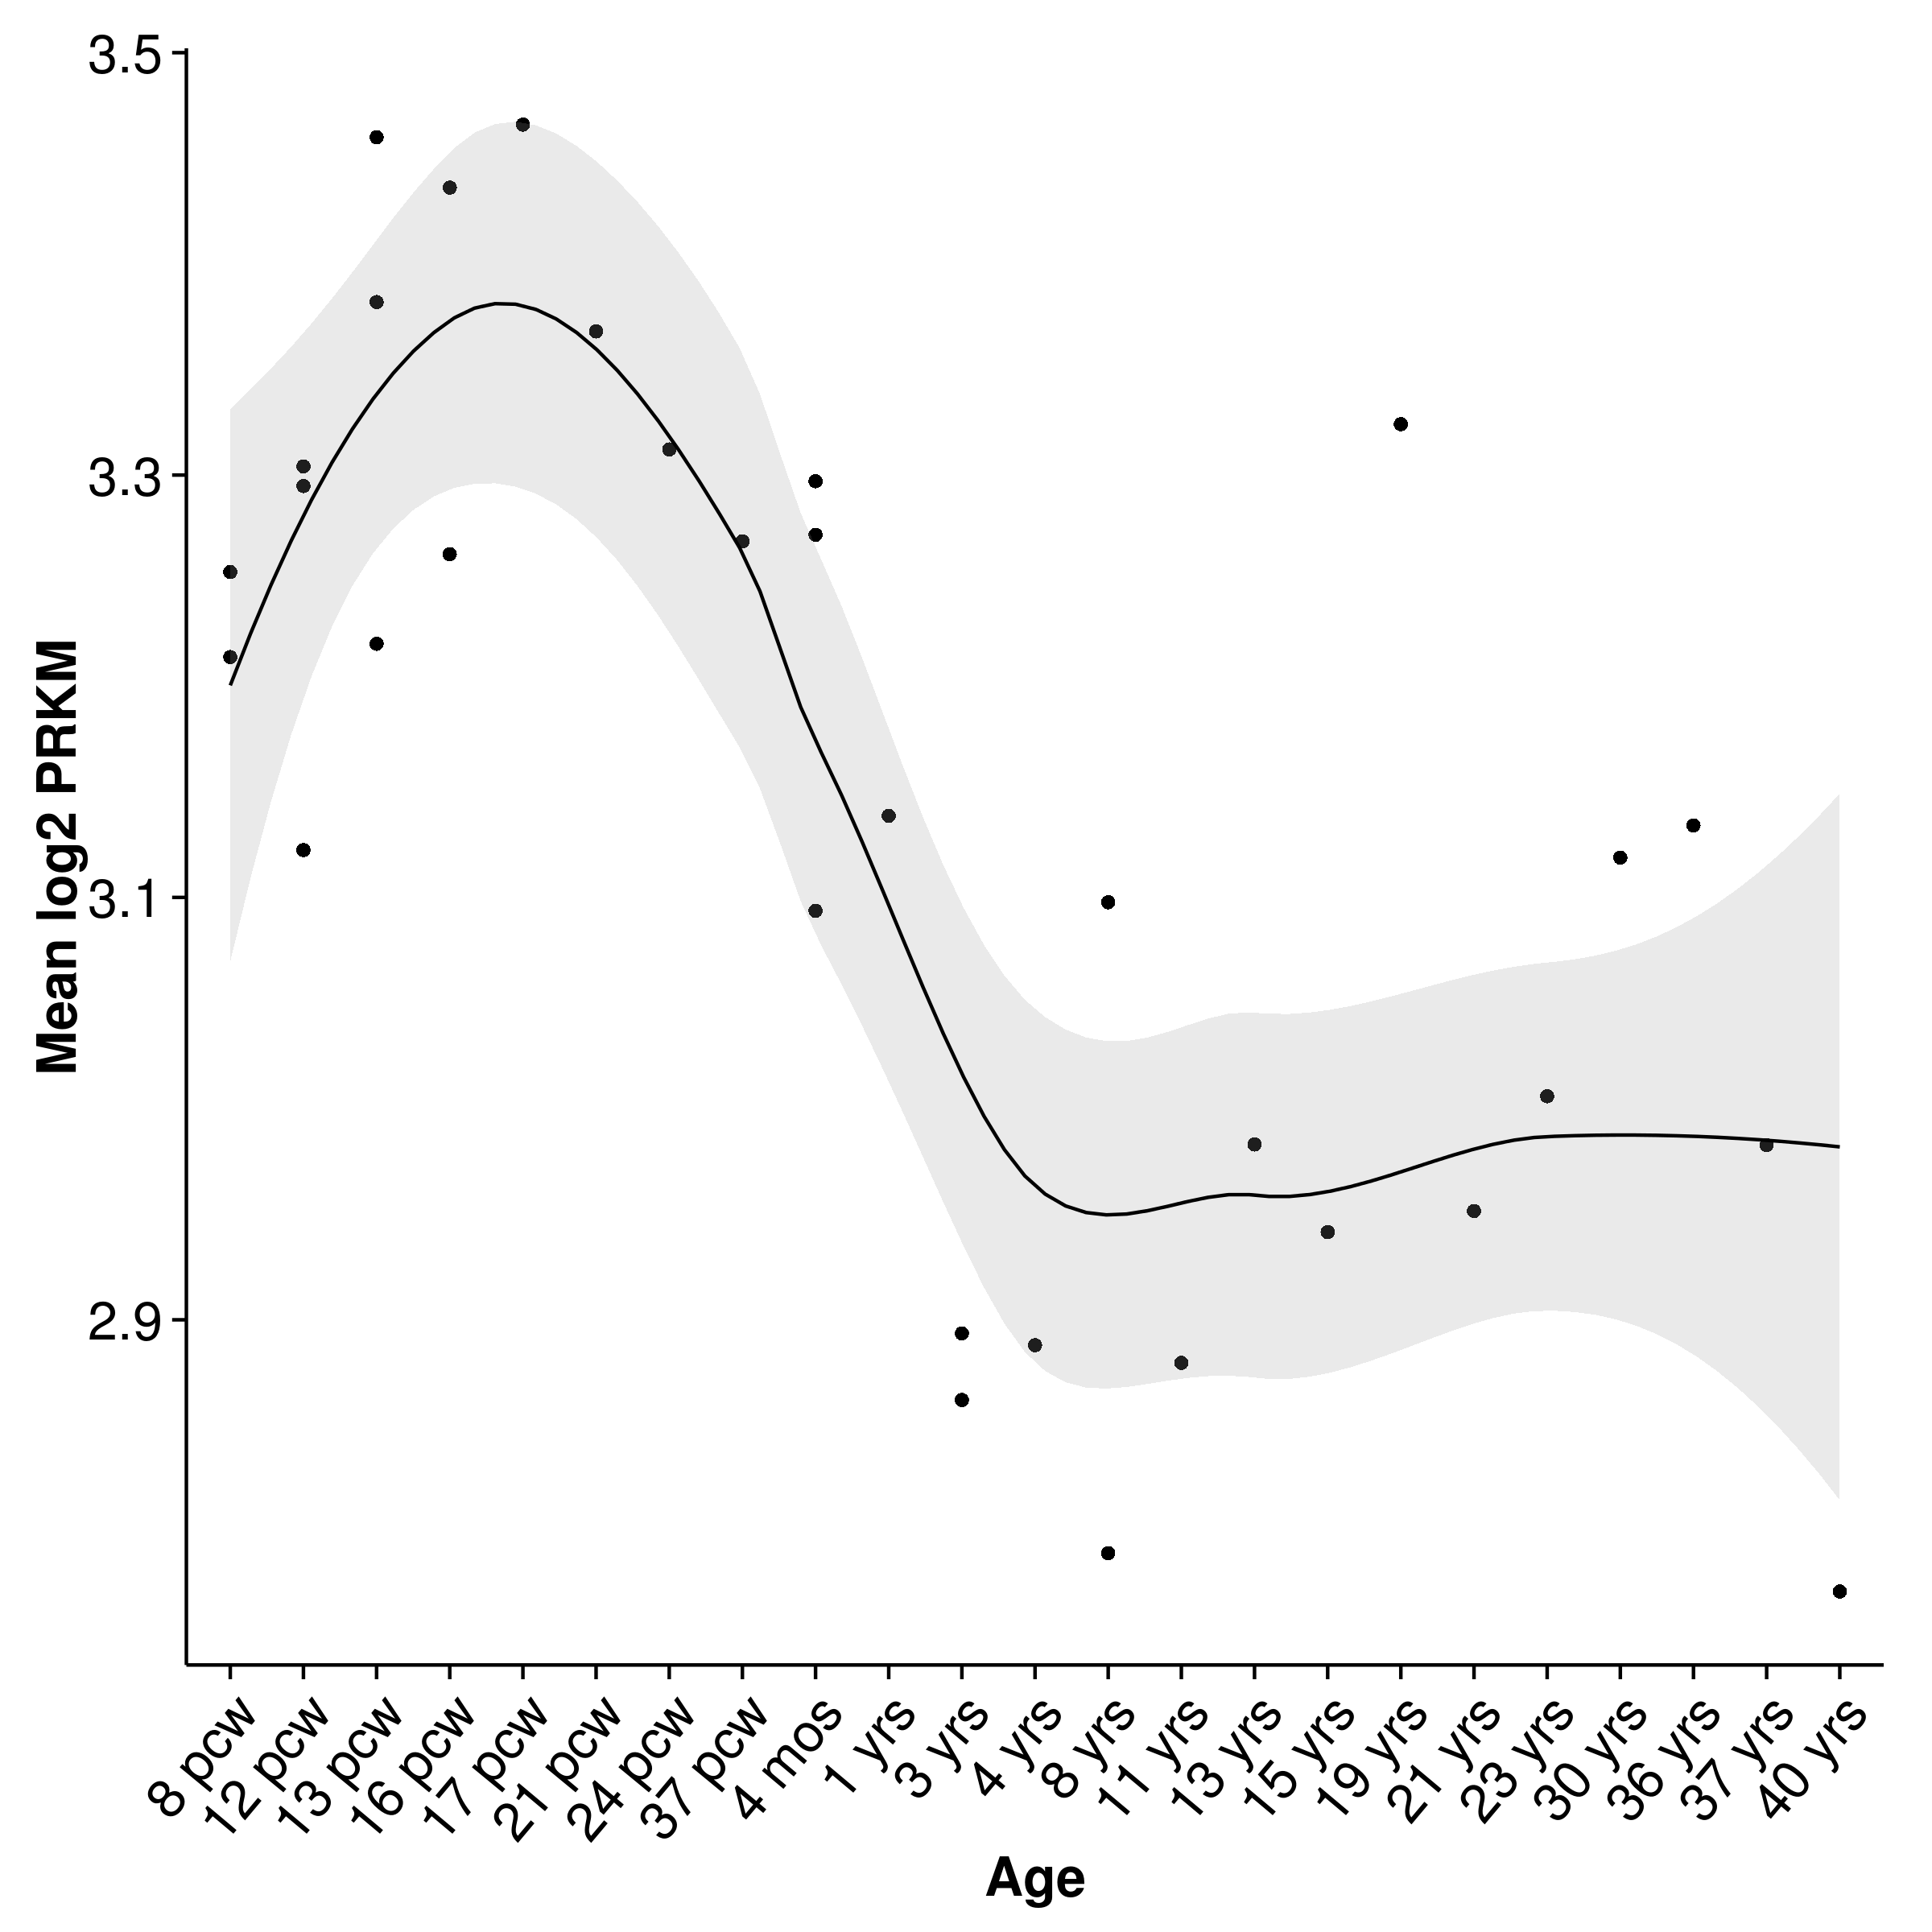
\includegraphics{figure/network/amy_pink_network}}
			\label{fig:pinkMod}
		}
		\subfloat[``Yellow'' Network from Amygdala]{
			\scalebox{.4}{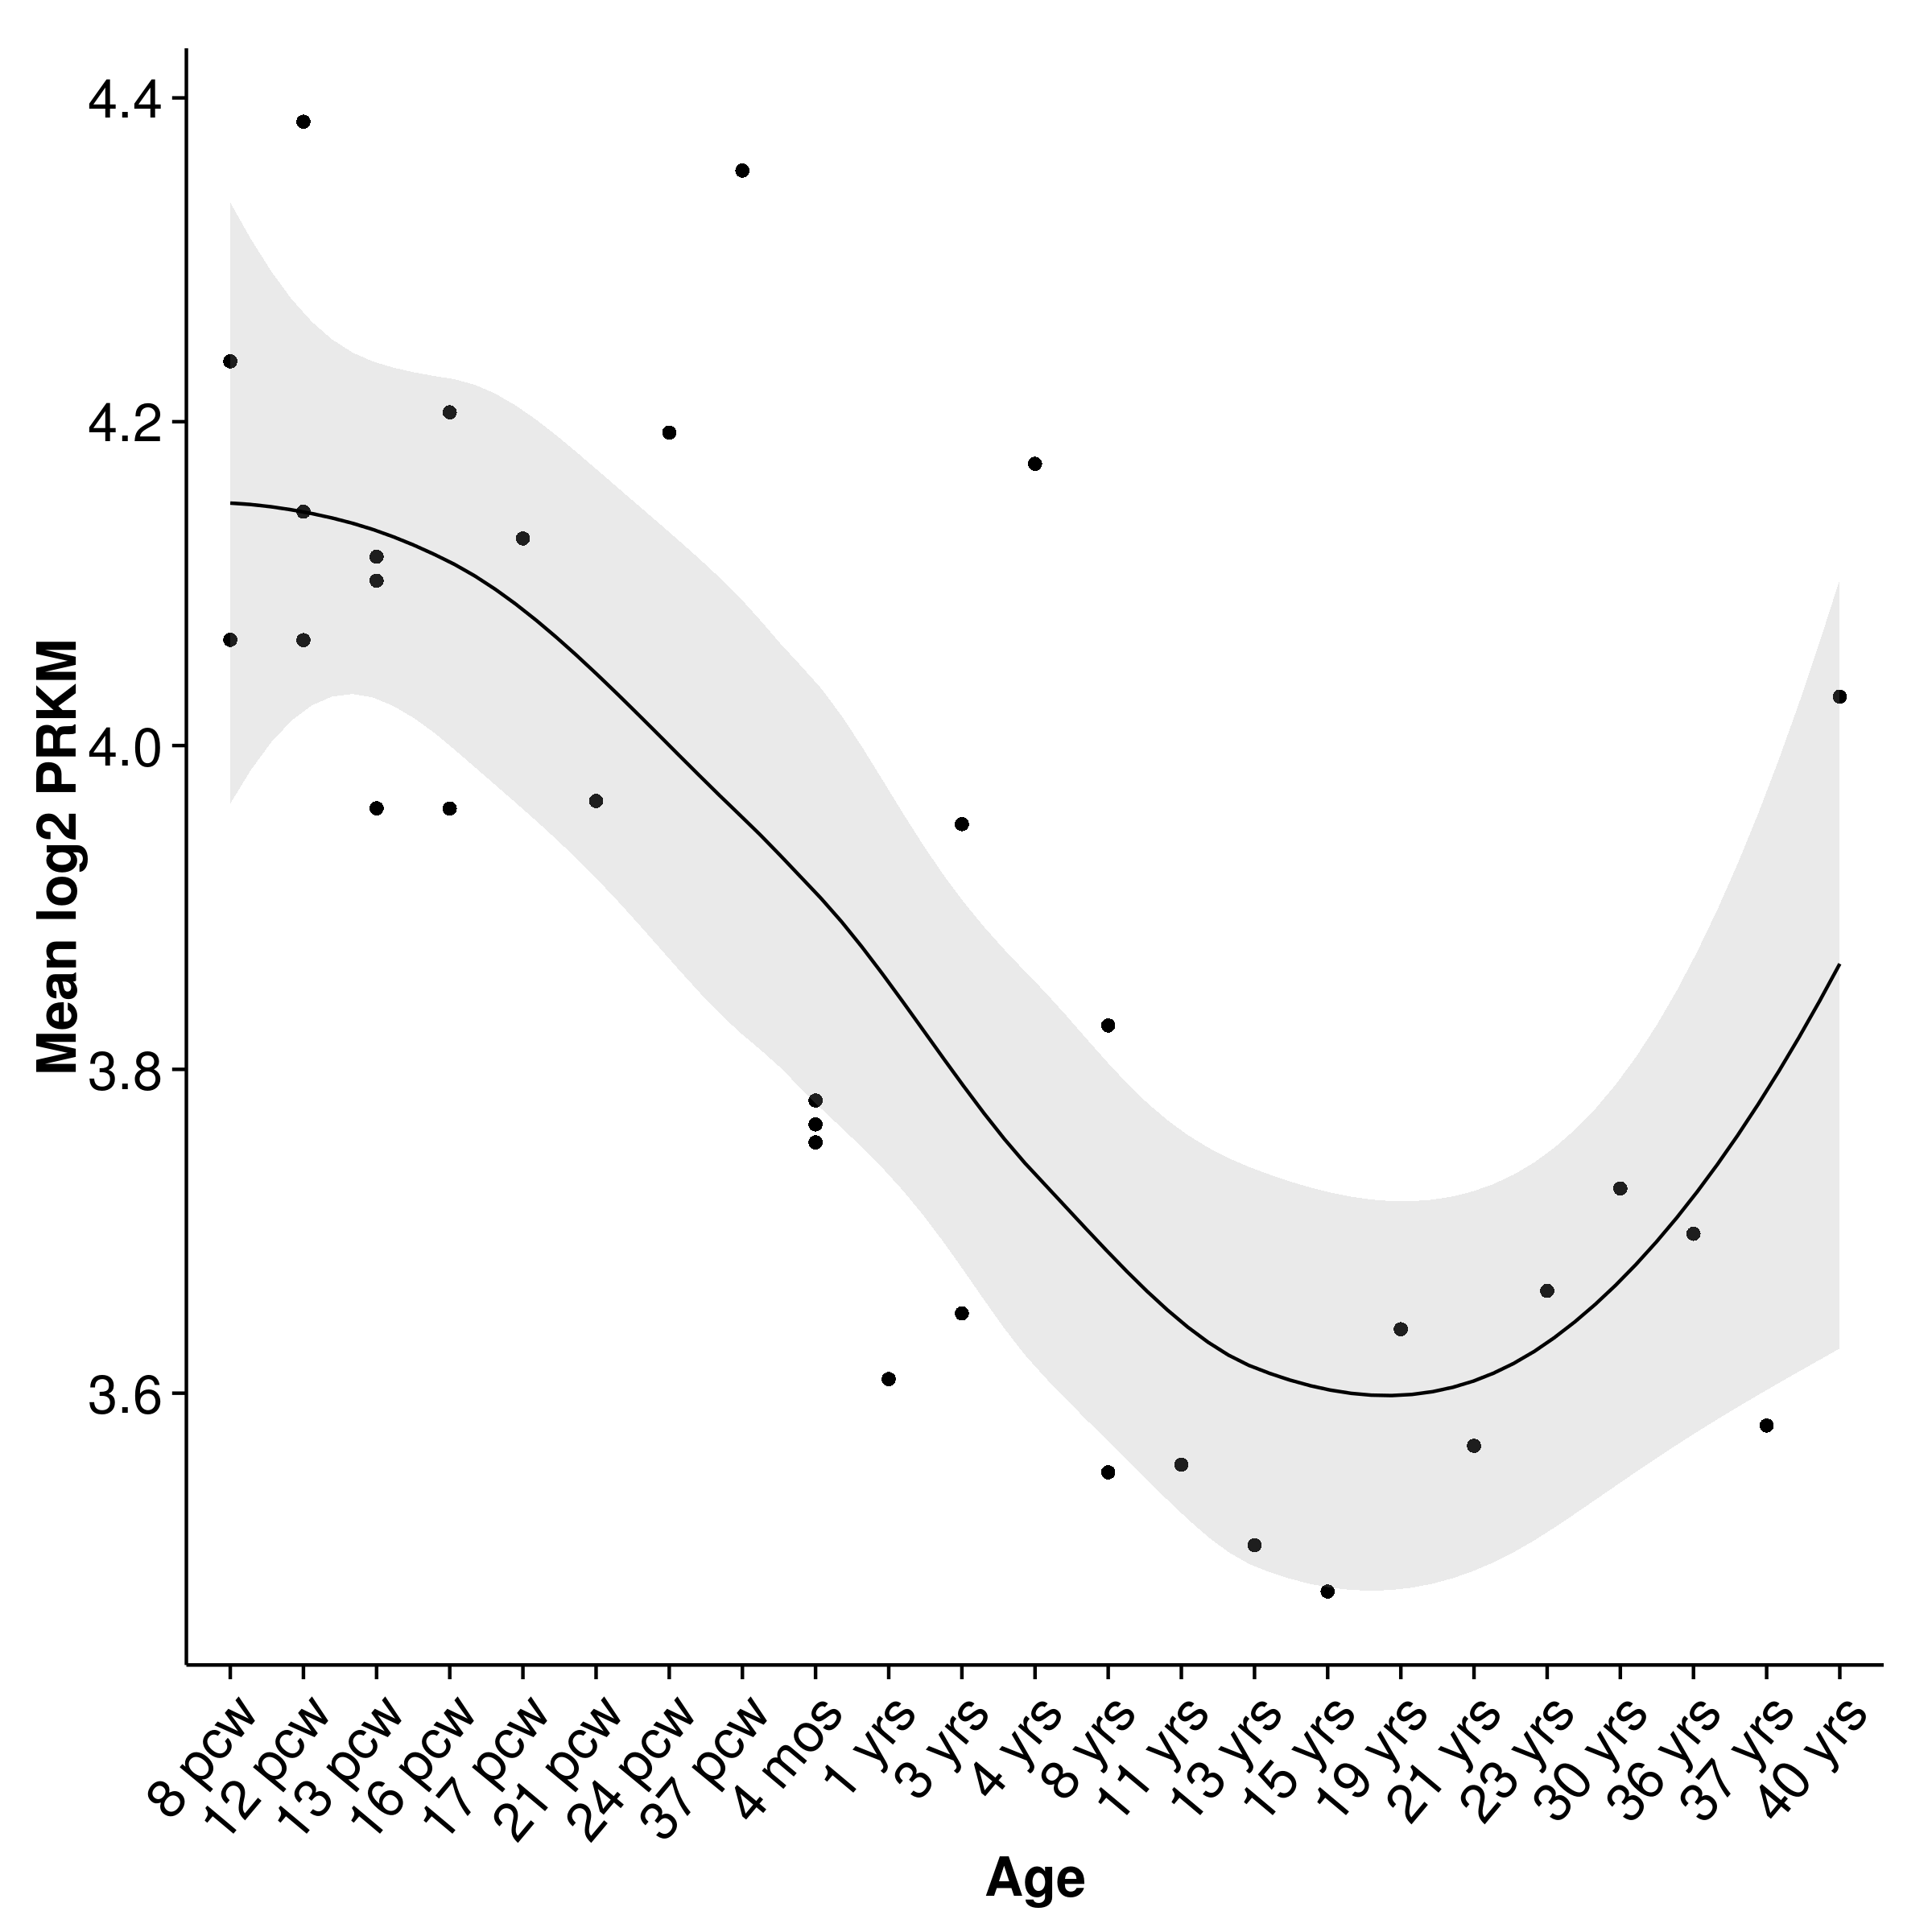
\includegraphics{figure/network/amy_yellow_network}}
			\label{fig:yellowMod}
		}
		\label{fig:allMod}
	\end{figure}
	
	
	
	\subsubsection{Functional Annotation}
	Upon performing the \gls{GO} enrichment analysis, a total of 16 \gls{GO} terms were enriched in the ``black'' hippocampus network, 4 in the ``tan'' amygdala network and 45 in the ``yellow'' amygdala network. 
	No \gls{GO} term was enriched in the ``pink'' amygdala network.
	
	The enriched \gls{GO} terms of the ``yellow'' amygdala network were mainly related to translation and transcription and were not specific to brain function or development(\cref{tab:yellowGO}). 
	On the contrary, the \gls{GO} terms enriched in the ``black'' hippocampus network were highly relevant to brain function and development (\cref{tab:blackGO})(e.g. ``central nervous system development'' and ``glutamate metabolic process'') and the ``tan'' amygdala network were also related to ammonium ion metabolism (\cref{tab:tanGO}) which is vita for glutamine synthesis from glutamate\citep{Liaw1995}. 
	
	Together, it is highly likely that the ``black'' hippocampus and ``tan'' amygdala networks are related to brain development and function.
	
	\begin{table}[h]
		\centering
		\caption[\glsentryshort{GO} enrichment results for the ``black'' network from Hippocampus]{\gls{GO} enrichment results for the ``black'' network from Hippocampus.
			Among the enriched \gls{GO} terms, it was most interesting to identify a number of brain developmental related \gls{GO} terms such as ``central nervous system development'', ``axon ensheathment in central nervous system'', ``glutamate metabolic process'' and ``positive regulation of gliogenesis''. 
			Surprisingly, \gls{GO} related to immune systems were also observed ``positive regulation of production of molecular mediator of immune response''.
		}
		\begin{tabular}{rrr}
			\toprule
			term\_ID & description & p-value \\
			\midrule
			GO:0019752 & carboxylic acid metabolic process & $4.92\times 10^{-6}$ \\
			GO:0007417 & central nervous system development & $5.94\times 10^{-5}$ \\
			GO:0002821 & positive regulation of adaptive immune response & $6.12\times 10^{-5}$ \\
			GO:0006082 & organic acid metabolic process & $1.03\times 10^{-3}$ \\
			GO:0032291 & axon ensheathment in central nervous system & $1.86\times 10^{-3}$ \\
			GO:1901565 & organonitrogen compound catabolic process & $1.99\times 10^{-3}$ \\
			GO:0006536 & glutamate metabolic process & $3.54\times 10^{-3}$ \\
			GO:0021762 & substantia nigra development & $3.73\times 10^{-3}$ \\
			GO:0044281 & small molecule metabolic process & $4.34\times 10^{-3}$ \\
			GO:0030194 & positive regulation of blood coagulation & $4.59\times 10^{-3}$ \\
			GO:0009607 & response to biotic stimulus & $6.14\times 10^{-3}$ \\
			GO:0002702 & positive regulation of production of molecular mediator of immune response & $6.21\times 10^{-3}$ \\
			GO:0034103 & regulation of tissue remodeling & $6.21\times 10^{-3}$ \\
			GO:0014015 & positive regulation of gliogenesis & $7.47\times 10^{-3}$ \\
			GO:0098542 & defense response to other organism & $7.95\times 10^{-3}$ \\
			GO:0019835 & cytolysis & $8.72\times 10^{-3}$ \\
			\bottomrule
		\end{tabular}%
		\label{tab:blackGO}%
	\end{table}%
	\begin{table}[h]
		\centering
		\caption[\glsentryshort{GO} enrichment results for the ``tan'' network from Amygdala]{\gls{GO} enrichment results for the ``tan'' network from Amygdala.
			Unlike the ``black'' network, only a small number of \gls{GO} terms were enriched. 
			However, these \gls{GO} terms are relatively specific to amine/ammonium ion metabolism.
			Interestingly, ammonium ion are essential to the synthesis of glutamine from glutamate, suggesting that this network might be relate to the glutamate system.
			}
		\begin{tabular}{rrr}
				\toprule
				term\_ID & description & p-value \\
				\midrule
				GO:0097164 & ammonium ion metabolic process & $1.37\times 10^{-3}$ \\
				GO:0044106 & cellular amine metabolic process & $4.2\times 10^{-3}$ \\
				GO:0009308 & amine metabolic process & $5.41\times 10^{-3}$ \\
				GO:0046519 & sphingoid metabolic process & $6.01\times 10^{-3}$ \\
				\bottomrule
		\end{tabular}%
		\label{tab:tanGO}%
	\end{table}%

	\subsubsection{Associate Co-expression network with \glsentryshort{pgc} schizophrenia data}
	Although the co-expression network were extremely interesting for their expression pattern and functional enrichment in brain development and function related \gls{GO} terms, there were no evidence of their involvement nor importance in schizophrenia.
	Therefore it is of particular interest for us to test whether if genes within these co-expression networks were associated withs schizophrenia. 
	
	First, gene base p-value of 18,622 genes were calculated using p-values from the \gls{pgc} schizophrenia working group\citep{Ripke2014}.
	Gene set enrichment analysis were then performed using \gls{MAGMA}\citep{DeLeeuw2015} to test whether if there genes within the ``black'' hippocampus and ``tan'' amygdala networks were significantly associated with schizophrenia.
	
	Based on the self-contained gene set enrichment analysis, genes within both networks were significantly associated with schizophrenia with p-value of $1.38\times 10^{-41}$ for the ``tan'' amygdala network and $2.70\times 10{-74}$ for the ``black'' hippocampus network.
	These suggest that these networks might be disrupted in schizophrenia patients.
	%Network	Size	self-contained	competitive
	%Amygdala        289   1.3869e-41      0.44715
	%Hippocampus     458   2.6993e-74      0.20002
	
	
	
	
	\subsubsection{Partitioning of Heritability}
	
	\section{Discussion}
	\chapter{Heritability of Response to antipsychotic treatment}
	\chaptermark{Response to antipsychotic treatment}
	%Maybe a section instead of a chapter?
	Important to schizophrenia research
	
	\section{Introduction}
	Here we try to use Beatrice's data and estimate the heritability explained in drug response.
	Should also repeat the region-wise heritability
	\section{Methodology}
	\section{Result}
	\section{Discussion}
	\chapter{Risk Prediction}
	\section{Methodology}
	We can define the traditional \gls{PGS} as
	\begin{equation}
	\hat{Y} = diag(\beta)X
	\end{equation}
	where $X$ is the standardized genotype, $\beta$ is the test-statistic calculated from other studies. 
	
	
	\subsection{Simulation}
	\section{Result}
	\section{Discussion}
	\chapter{Conclusion}
	
	
	
	
	
	
	
	
	\backmatter
	\printbibliography
	\chapter*{Supplementary Materials}
	\beginsupplement
	\begin{table}[htbp]
		\centering
		\caption[\glsentryshort{GO} enrichment results for the ``yellow'' network from Amygdala]{\gls{GO} enrichment results for the ``yellow'' network from Amygdala. 
			Most of the terms are related to translation transcription and are not specific enough to understand the true function of the network}
		\begin{tabular}{rrr}
			\toprule
			term\_ID & description & p-value \\
			\midrule
			GO:0006614 & SRP-dependent cotranslational protein targeting to membrane & $1.63\times 10^{-47}$ \\
			GO:0006412 & translation & $5.76\times 10^{-27}$ \\
			GO:0006171 & cAMP biosynthetic process & $1.5\times 10^{-3}$ \\
			GO:0042274 & ribosomal small subunit biogenesis & $3.13\times 10^{-8}$ \\
			GO:0006413 & translational initiation & $2.12\times 10^{-28}$ \\
			GO:0006414 & translational elongation & $7.63\times 10^{-31}$ \\
			GO:0006415 & translational termination & $3.92\times 10^{-32}$ \\
			GO:0071702 & organic substance transport & $4.16\times 10^{-10}$ \\
			GO:0002181 & cytoplasmic translation & $1.19\times 10^{-7}$ \\
			GO:1901566 & organonitrogen compound biosynthetic process & $6\times 10^{-17}$ \\
			GO:0070972 & protein localization to endoplasmic reticulum & $5.36\times 10^{-44}$ \\
			GO:0071822 & protein complex subunit organization & $2.21\times 10^{-6}$ \\
			GO:0071826 & ribonucleoprotein complex subunit organization & $3.67\times 10^{-3}$ \\
			GO:0022411 & cellular component disassembly & $1.55\times 10^{-17}$ \\
			GO:1902578 & single-organism localization & $4.3\times 10^{-8}$ \\
			GO:1902580 & single-organism cellular localization & $1.3\times 10^{-15}$ \\
			GO:0000028 & ribosomal small subunit assembly & $1.91\times 10^{-7}$ \\
			GO:0033036 & macromolecule localization & $1.74\times 10^{-11}$ \\
			GO:0070727 & cellular macromolecule localization & $1.09\times 10^{-16}$ \\
			GO:0006605 & protein targeting & $1.64\times 10^{-28}$ \\
			GO:0022613 & ribonucleoprotein complex biogenesis & $3.32\times 10^{-9}$ \\
			GO:0044765 & single-organism transport & $4.19\times 10^{-8}$ \\
			GO:0044085 & cellular component biogenesis & $4.81\times 10^{-7}$ \\
			GO:0061024 & membrane organization & $5.29\times 10^{-15}$ \\
			GO:0051641 & cellular localization & $1.65\times 10^{-14}$ \\
			GO:0044267 & cellular protein metabolic process & $6.57\times 10^{-5}$ \\
			GO:0019083 & viral transcription & $1.64\times 10^{-44}$ \\
			GO:1901564 & organonitrogen compound metabolic process & $1.15\times 10^{-14}$ \\
			GO:0019538 & protein metabolic process & $4.17\times 10^{-5}$ \\
			GO:0006401 & RNA catabolic process & $1.34\times 10^{-29}$ \\
			GO:0010467 & gene expression & $1.4\times 10^{-11}$ \\
			GO:0044419 & interspecies interaction between organisms & $4.74\times 10^{-15}$ \\
			GO:0043604 & amide biosynthetic process & $4.35\times 10^{-26}$ \\
			GO:0043603 & cellular amide metabolic process & $4.94\times 10^{-21}$ \\
			GO:0044764 & multi-organism cellular process & $1.11\times 10^{-15}$ \\
			GO:0016072 & rRNA metabolic process & $2.03\times 10^{-3}$ \\
			GO:0016071 & mRNA metabolic process & $1.58\times 10^{-15}$ \\
			GO:0000184 & nuclear-transcribed mRNA catabolic process, nonsense-mediated decay & $4.81\times 10^{-42}$ \\
			GO:0034655 & nucleobase-containing compound catabolic process & $1.29\times 10^{-24}$ \\
			GO:0044699 & single-organism process & $2.4\times 10^{-5}$ \\
			GO:0051179 & localization & $7.96\times 10^{-8}$ \\
			GO:0051704 & multi-organism process & $6.02\times 10^{-12}$ \\
			GO:0071840 & cellular component organization or biogenesis & $3.83\times 10^{-3}$ \\
			GO:0048871 & multicellular organismal homeostasis & $6.56\times 10^{-3}$ \\
			GO:0009056 & catabolic process & $1.8\times 10^{-11}$ \\
			\bottomrule
		\end{tabular}%
		\label{tab:yellowGO}%
	\end{table}%

	\chapter*{Appendix}

\end{document}


